\documentclass[11pt,a4paper]{ctexart}
\usepackage{geometry}
\geometry{margin=2cm}
\usepackage{amsmath}
\usepackage{amssymb}
\usepackage{extarrows}
\usepackage{amsthm}
\usepackage{mathtools}
\usepackage{bm}
\usepackage{graphicx}
\usepackage{tikz}
\usepackage{titlesec}
\usepackage{hyperref}
\usepackage[type={CC},modifier={by},version={4.0}]{doclicense}

\usetikzlibrary{arrows.meta}

\newcommand{\sectionbreak}{\clearpage}

\newtheorem*{lemma}{Lemma}
\newtheorem*{theorem}{Theorem}

\begin{document}

\title{浅谈矩阵微积分}
\author{evilayuria \thanks{WeChat: \texttt{autoLambda8080}, \quad Email: \texttt{lqwql4x@gmail.com}}}
\date{\today}

\maketitle

\begin{center}
\doclicenseThis
\end{center}

\begin{center}
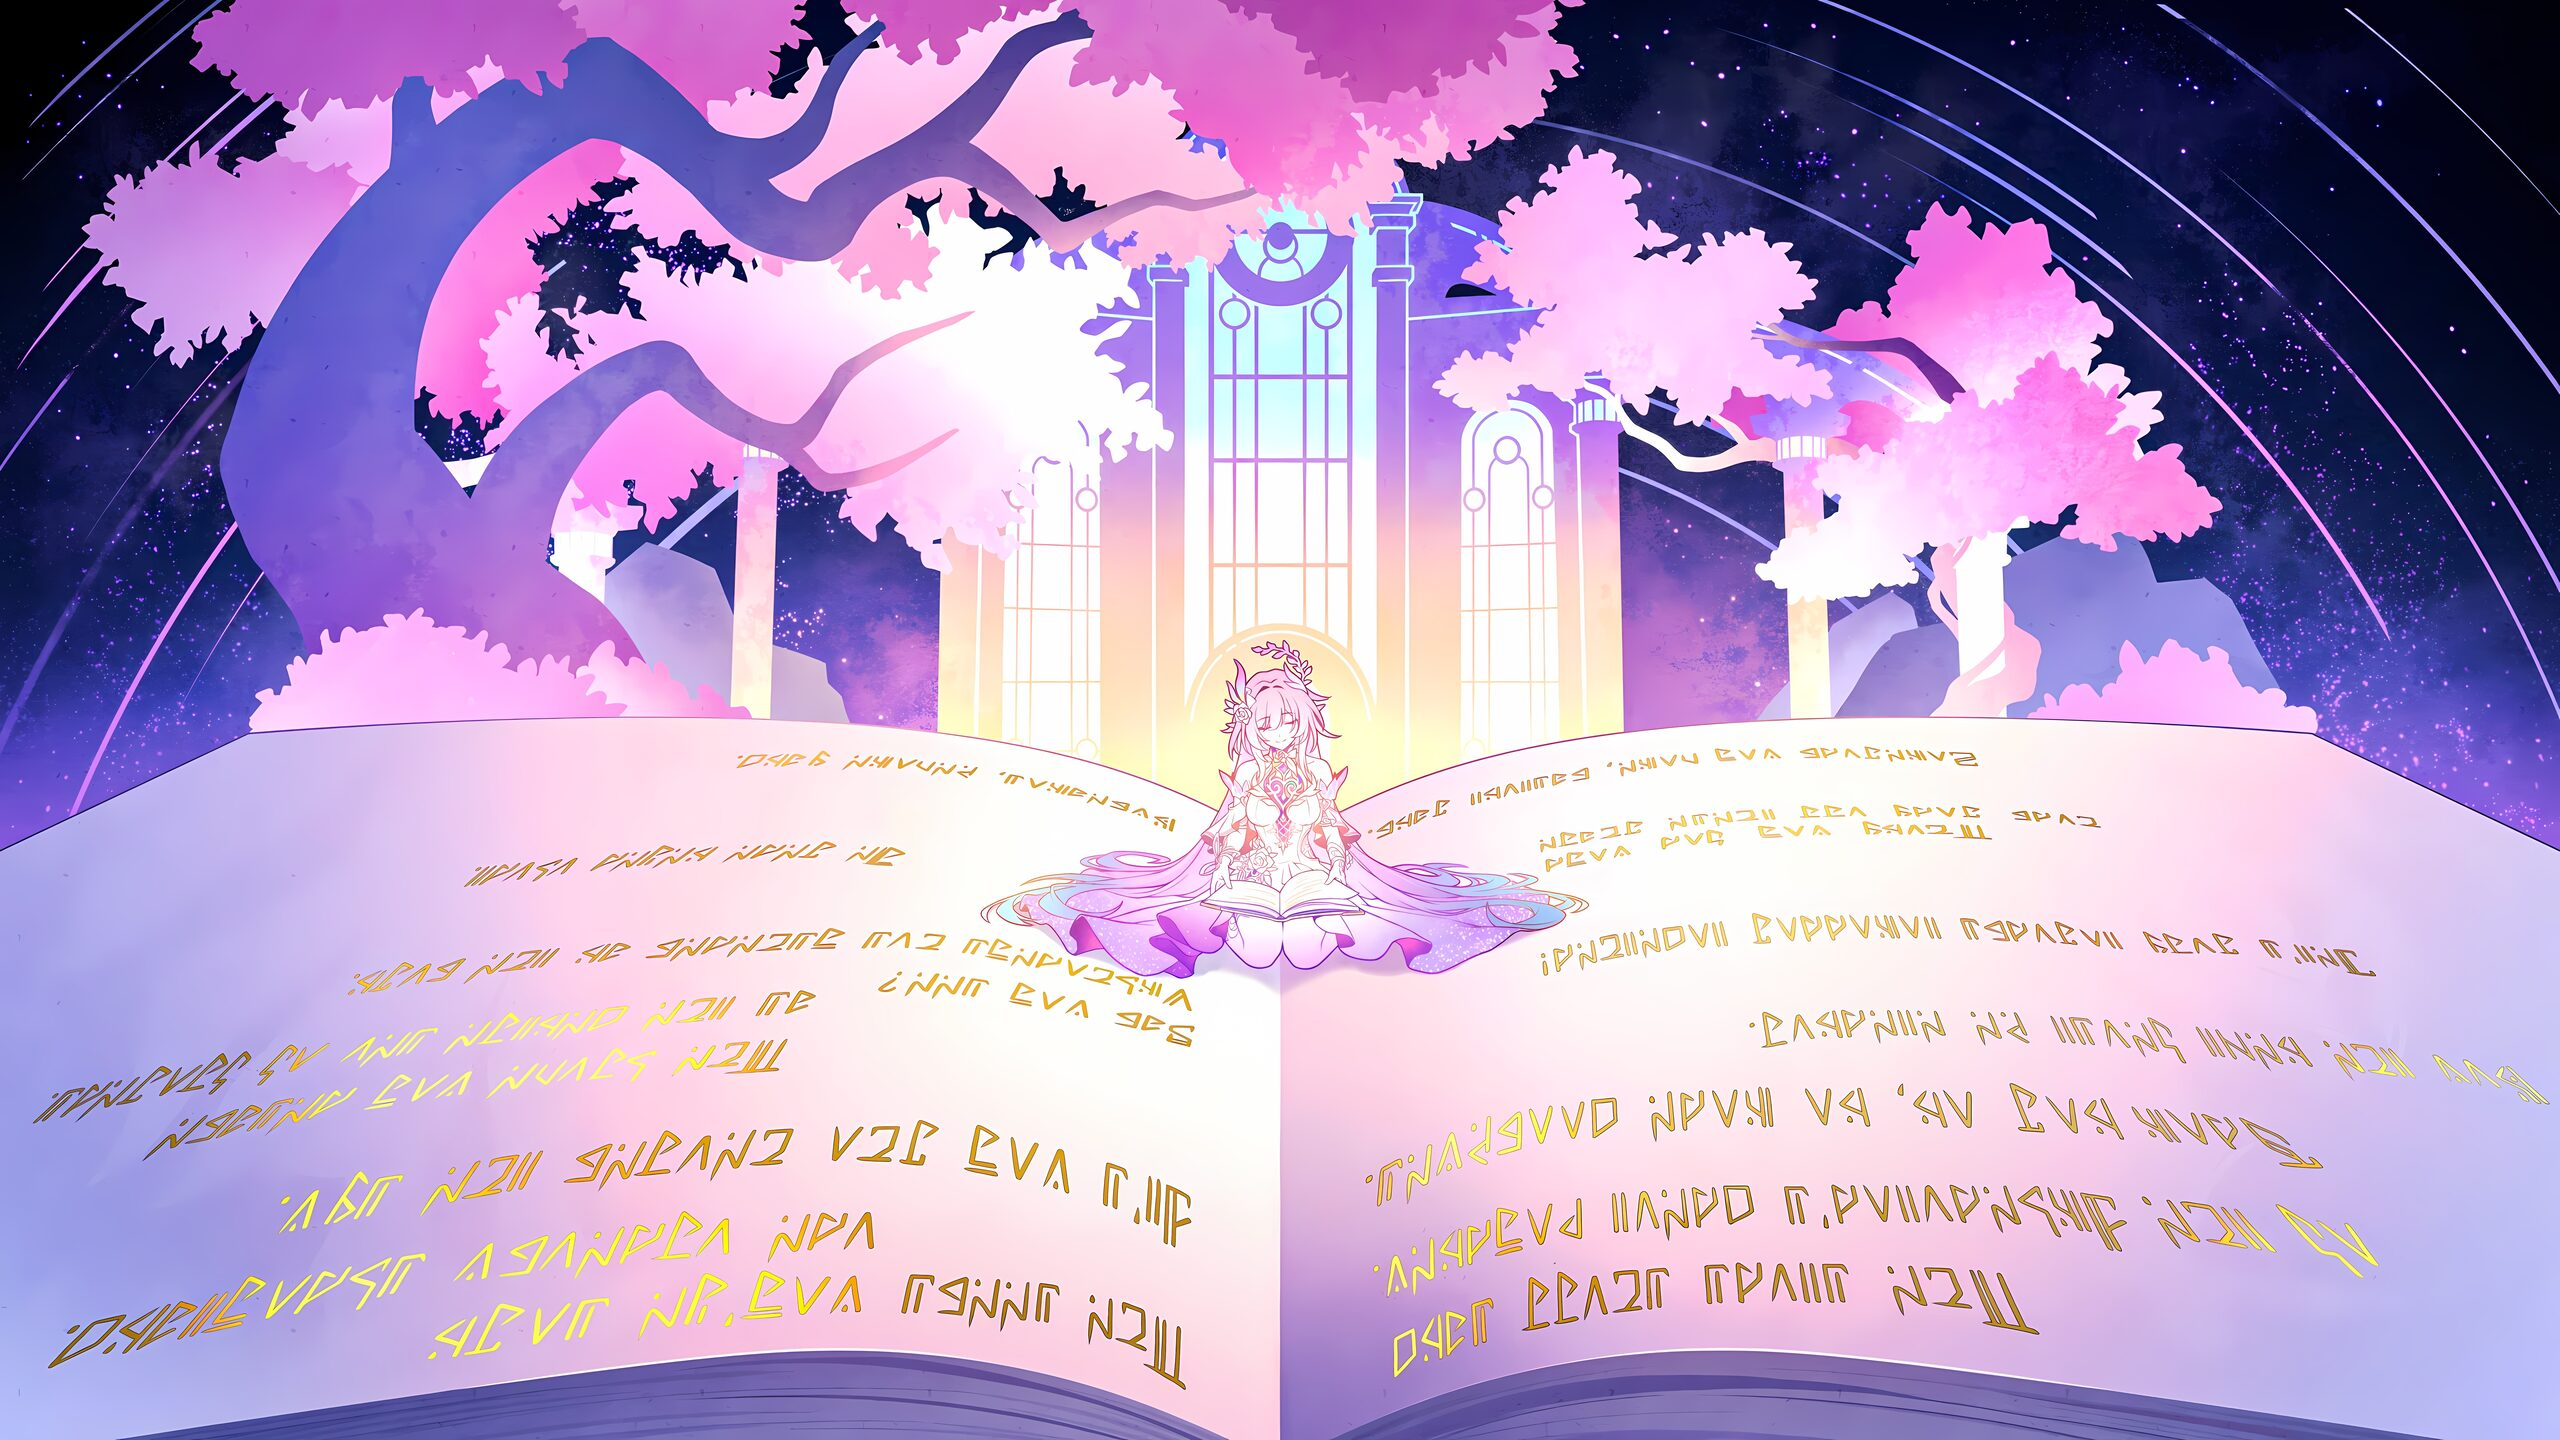
\includegraphics[width=\textwidth,height=0.62\textheight,keepaspectratio]{assets/before.png}
\end{center}

\tableofcontents

\section{一元函数、多元函数的局部线性近似}

\begin{center}
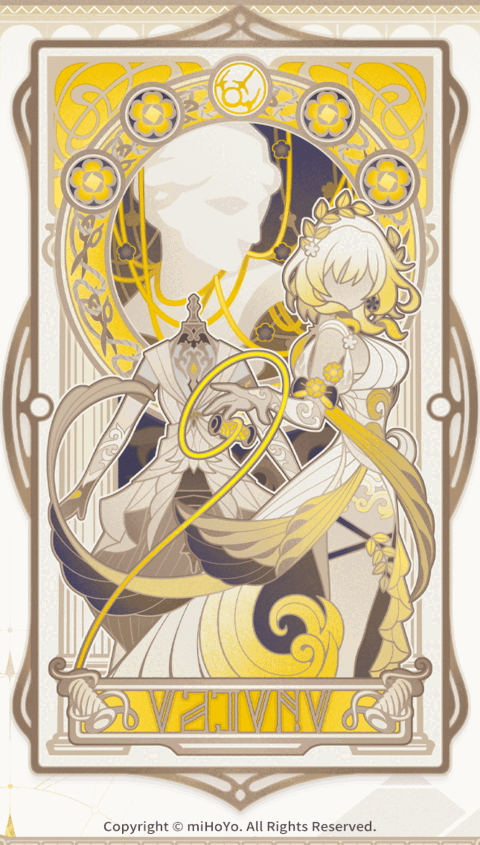
\includegraphics[width=0.22\textwidth]{assets/hsr_coreflame_icons/Icon_Coreflame_Romance.png}
\end{center}

函数的求导问题首先来自一个基本要求：当输入发生很小改变时，函数值随之发生怎样的主要改变。对于一元函数 \(f:\mathbb{R}\to\mathbb{R}\)，若在点 \(x\) 处可导，则当输入由 \(x\) 变为 \(x+h\) 时，函数增量可以写成
\[
f(x+h)-f(x)=f'(x)h+o(|h|),\qquad h\to 0.
\]
其中 \(h\) 是输入增量，\(f'(x)h\) 是关于 \(h\) 的线性主项，\(o(|h|)\) 是比 \(|h|\) 更高阶的小量。导数 \(f'(x)\) 不仅表示切线斜率，也确定输入小增量 \(h\) 对函数值主要增量的贡献方式。

以 \(f(x)=x^2\) 为例，直接展开得到
\[
f(x+h)-f(x)=(x+h)^2-x^2=2xh+h^2.
\]
当 \(h\to 0\) 时，\(h^2=o(|h|)\)，因此一阶主项为 \(2xh\)，导数为 \(f'(x)=2x\)。在这个计算中，常数项 \(f(x)\) 表示基点处的函数值，线性项 \(2xh\) 描述局部主要变化，二次项 \(h^2\) 则被归入余项。

线性函数是最简单的情形。若 \(f(x)=ax+b\)，则 \(f(x+h)-f(x)=ah\)，没有更高阶余项，函数在每一点的局部变化完全由线性项决定。与此相比，非线性函数没有这么好的性质，但在局部我们可以用线性项来做近似，只要余项相对于 \(|h|\) 足够小，一阶主项仍然决定函数值的主要改变。

这一观点在多元函数中保持不变，只是输入增量由数 \(h\) 变为向量 \(\bm{u}\)。设 \(f:\mathbb{R}^n\to\mathbb{R}\)，点 \(\bm{x}\in\mathbb{R}^n\) 附近的输入改变量为 \(\bm{u}\in\mathbb{R}^n\)。若 \(f\) 在 \(\bm{x}\) 处可微，则函数增量满足
\[
f(\bm{x}+\bm{u})-f(\bm{x})=\bm{\nabla} f(\bm{x})^\top \bm{u}+o(\|\bm{u}\|),\qquad \bm{u}\to \bm{0}.
\]
这里 \(\bm{\nabla} f(\bm{x})\in\mathbb{R}^n\) 是梯度，\(\bm{\nabla} f(\bm{x})^\top \bm{u}\) 是关于向量增量 \(\bm{u}\) 的线性主项，余项 \(o(\|\bm{u}\|)\) 在 \(\bm{u}\) 趋于零时比 \(\|\bm{u}\|\) 更小。这个公式把一元情形中的 \(f'(x)h\) 推广为向量内积形式，说明多元函数的一阶变化由输入方向 \(\bm{u}\) 与梯度 \(\bm{\nabla} f(\bm{x})\) 的配对决定。

对于线性函数 \(f(\bm{x})=\bm{a}^\top \bm{x}\)，其中 \(\bm{a}\in\mathbb{R}^n\)，有
\[
f(\bm{x}+\bm{u})-f(\bm{x})=\bm{a}^\top(\bm{x}+\bm{u})-\bm{a}^\top \bm{x}=\bm{a}^\top \bm{u}.
\]
因此 \(\bm{\nabla} f(\bm{x})=\bm{a}\)，且该梯度与点 \(\bm{x}\) 无关。梯度可以被理解为线性主项的系数向量；当输入改变量为 \(\bm{u}\) 时，函数值的主要改变量由向量 \(\bm{a}\) 与 \(\bm{u}\) 的内积表示。

二次型保留了非线性多元函数中的同一结构。设 \(A\in\mathbb{R}^{n\times n}\)，考虑 \(f(\bm{x})=\bm{x}^\top A\bm{x}\)。直接展开可得
\[
f(\bm{x}+\bm{u})-f(\bm{x})=(\bm{x}+\bm{u})^\top A(\bm{x}+\bm{u})-\bm{x}^\top A\bm{x}
=\bm{x}^\top A\bm{u}+\bm{u}^\top A\bm{x}+\bm{u}^\top A\bm{u}.
\]
由于 \(\bm{x}^\top A\bm{u}=(A^\top \bm{x})^\top \bm{u}\)，且 \(\bm{u}^\top A\bm{x}=(A\bm{x})^\top \bm{u}\)，所以上式的一阶主项为 \(((A+A^\top)\bm{x})^\top \bm{u}\)，二次项 \(\bm{u}^\top A\bm{u}\) 是 \(O(\|\bm{u}\|^2)\)，从而属于 \(o(\|\bm{u}\|)\)。因此
\[
f(\bm{x}+\bm{u})-f(\bm{x})=((A+A^\top)\bm{x})^\top \bm{u}+o(\|\bm{u}\|),
\]
并得到 \(\bm{\nabla} f(\bm{x})=(A+A^\top)\bm{x}\)。若 \(A\) 是对称矩阵，则梯度化为 \(2A\bm{x}\)。

这些例子指向同一个计算重点：从函数增量中识别关于输入增量的线性主项。一元情形中，这个主项形如 \(f'(x)h\)；多元标量函数中，这个主项形如 \(\bm{\nabla} f(\bm{x})^\top \bm{u}\)。导数和梯度记录了局部线性近似的系数，使复杂函数在小范围内可以被线性函数替代。

这种替代必须同时保留两个信息。

\begin{enumerate}
    \item 第一，线性主项依赖于基点，例如 \(x^2\) 在 \(x\) 处的一阶系数为 \(2x\)，二次型 \(\bm{x}^\top A\bm{x}\) 在 \(\bm{x}\) 处的一阶系数为 \((A+A^\top)\bm{x}\)。
    \item 第二，线性主项作用于输入增量，例如 \(2xh\) 中真正描述变化的是 \(h\mapsto 2xh\)，\(\bm{\nabla} f(\bm{x})^\top \bm{u}\) 中真正描述变化的是 \(\bm{u}\mapsto \bm{\nabla} f(\bm{x})^\top \bm{u}\)。若只记住 \(f'(x)\) 或 \(\bm{\nabla} f(\bm{x})\) 本身，而忽略它们与输入增量的配对，就容易把导数误认为一个孤立对象。
\end{enumerate}

局部线性近似也解释了梯度在优化中的基本作用。若 \(f:\mathbb{R}^n\to\mathbb{R}\) 在 \(\bm{x}\) 处可微，则沿方向 \(\bm{u}\) 的一阶变化为 \(\bm{\nabla} f(\bm{x})^\top \bm{u}\)。当 \(\bm{\nabla} f(\bm{x})\ne \bm{0}\) 时，选择 \(\bm{u}=-\bm{\nabla} f(\bm{x})\) 会使一阶主项为 \(-\|\bm{\nabla} f(\bm{x})\|^2\)，因此函数值在这个方向上首先呈下降趋势；若 \(\bm{x}\) 是无约束局部极小点，则任意小方向上的一阶主项都不能产生下降趋势，因而必须满足 \(\bm{\nabla} f(\bm{x})=\bm{0}\)。这个结论直接来自同一个增量公式，不需要引入额外的优化规则。

\section{微分是一种线性映射}

\begin{center}
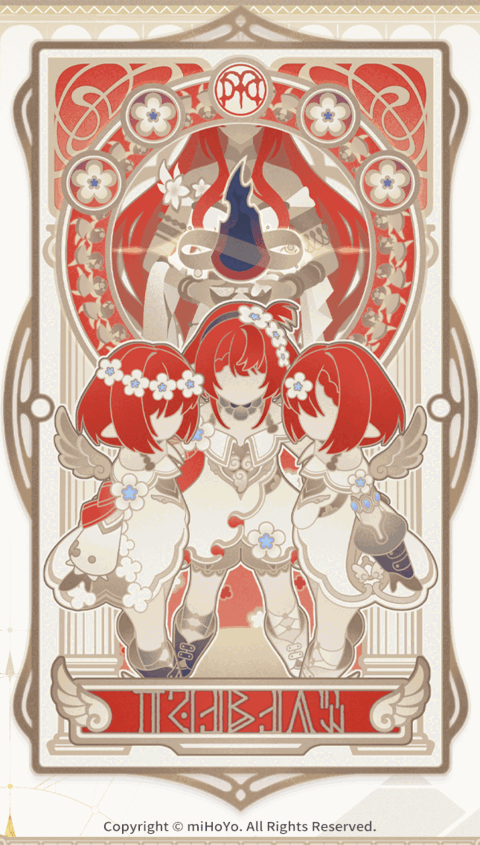
\includegraphics[width=0.22\textwidth]{assets/hsr_coreflame_icons/Icon_Coreflame_Passage.png}
\end{center}

回顾函数的局部展开，它们都有同一种形式：函数在基点处的值保持不变，输入增量产生一个线性主项，其余部分相对于增量范数更高阶。对于一元函数，这个结构写作 \[f(x+h)=f(x)+f'(x)h+o(|h|),\] 对于多元标量函数，这个结构写作 \[f(\bm{x}+\bm{u})=f(\bm{x})+\bm{\nabla} f(\bm{x})^\top \bm{u}+o(\|\bm{u}\|).\]
两式中的 \(f'(x)h\) 与 \(\bm{\nabla} f(\bm{x})^\top \bm{u}\) 承担相同功能，都是把输入增量送到函数增量的一阶主项。

为了把这种功能从具体坐标公式中分离出来，设 \(f:\mathbb{R}^n\to\mathbb{R}\)，若存在一个关于 \(\bm{u}\) 的线性规则，使得
\[
f(\bm{x}+\bm{u})=f(\bm{x})+\mathrm{D}f(\bm{x})[\bm{u}]+o(\|\bm{u}\|),\qquad \bm{u}\to \bm{0},
\]
则称 \(f\) 在 \(\bm{x}\) 处\textbf{可微}，并把 \(\mathrm{D}f(\bm{x})\) 称为 \(f\) 在 \(\bm{x}\) 处的\textbf{微分}。这里 \(\mathrm{D}f(\bm{x})[\bm{u}]\) 表示这个规则作用在输入增量 \(\bm{u}\) 上得到的数值，而 \(\mathrm{D}f(\bm{x})\) 本身表示从输入增量到一阶主项的对应关系。方括号中的 \(\bm{u}\) 表示函数自变量在 \(\bm{x}\) 附近发生的改变量。

在一元情形中，输入增量是实数 \(h\)，微分为
\[
\mathrm{D}f(x)[h]=f'(x)h.
\]
因此，导数 \(f'(x)\) 是这个线性映射的系数，而微分 \(\mathrm{D}f(x)\) 是把 \(h\) 映到 \(f'(x)h\) 的作用方式。若只写 \(f'(x)\)，得到的是一个数；若写 \(\mathrm{D}f(x)[h]\)，得到的是该数与输入增量配对后的函数增量主项。这一区分在一元函数中显得简单，但在多元和矩阵变量情形中会成为组织公式的关键。

对于多元标量函数，若 \(f\) 在 \(\bm{x}\) 处可微，采用欧氏内积，则微分可以写为
\[
\mathrm{D}f(\bm{x})[\bm{u}]=\bm{\nabla} f(\bm{x})^\top \bm{u}.
\]
梯度是在欧氏内积下表示微分规则的向量，而微分本身是关于输入增量 \(\bm{u}\) 的线性映射。由于这一表示依赖于内积约定，进入矩阵空间时必须先明确采用哪一种内积，才能从微分中读出梯度。

多元微积分中常见的偏导公式正是这个线性映射的坐标表达。把 \(\bm{u}=(u_1,\ldots,u_n)^\top\) 写成 \(\bm{u}=\sum_i u_i \bm{e}_i\)，其中 \(\bm{e}_i\) 是第 \(i\) 个标准基向量。若 \(\mathrm{D}f(\bm{x})\) 是线性映射，则
\[
\mathrm{D}f(\bm{x})[\bm{u}]=\sum_i u_i \mathrm{D}f(\bm{x})[\bm{e}_i].
\]
而 \(\mathrm{D}f(\bm{x})[\bm{e}_i]\) 正是函数沿第 \(i\) 个坐标方向的一阶系数，也就是偏导数 \(\frac{\partial f}{\partial x_i}(\bm{x})\)。因此
\[
\mathrm{D}f(\bm{x})[\bm{u}]=\sum_i \frac{\partial f}{\partial x_i}(\bm{x})u_i=\bm{\nabla} f(\bm{x})^\top \bm{u}.
\]
于是，偏导数应理解为全微分在标准坐标方向上的系数；梯度把这些系数排成向量，内积形式则把它们对任意增量 \(\bm{u}\) 的作用一次性写出。

线性函数 \(f(\bm{x})=\bm{a}^\top \bm{x}+b\) 是最简单的例子。对任意 \(\bm{u}\in\mathbb{R}^n\)，有
\[
f(\bm{x}+\bm{u})-f(\bm{x})=\bm{a}^\top \bm{u},
\]
因此 \(\mathrm{D}f(\bm{x})[\bm{u}]=\bm{a}^\top \bm{u}\)，且微分与基点 \(\bm{x}\) 无关。这里的函数本身已经是线性的，局部展开没有高阶余项。

二次型 \(f(\bm{x})=\bm{x}^\top A\bm{x}\) 则显示了微分怎样从非线性函数中提取局部线性部分。由前面的展开可知
\[
f(\bm{x}+\bm{u})-f(\bm{x})=\bm{x}^\top A\bm{u}+\bm{u}^\top A\bm{x}+\bm{u}^\top A\bm{u}.
\]
其中前两项关于 \(\bm{u}\) 线性，最后一项是二阶小量。因此
\[
\mathrm{D}f(\bm{x})[\bm{u}]=\bm{x}^\top A\bm{u}+\bm{u}^\top A\bm{x}=((A+A^\top)\bm{x})^\top \bm{u}.
\]
这个式子同时包含两个信息：作为微分，\(\mathrm{D}f(\bm{x})\) 是把 \(\bm{u}\) 映到 \(\bm{x}^\top A\bm{u}+\bm{u}^\top A\bm{x}\) 的线性映射；作为梯度表示，它对应于向量 \(\bm{\nabla} f(\bm{x})=(A+A^\top)\bm{x}\)。若 \(A=A^\top\)，这个表示才进一步化为 \(\bm{\nabla} f(\bm{x})=2A\bm{x}\)。

微分记号的优势在于它直接记录函数复合、相加和相乘时一阶主项的来源。若 \(f,g:\mathbb{R}^n\to\mathbb{R}\) 都在 \(\bm{x}\) 处可微，则
\[
\mathrm{D}(f+g)(\bm{x})[\bm{u}]=\mathrm{D}f(\bm{x})[\bm{u}]+\mathrm{D}g(\bm{x})[\bm{u}].
\]
这是因为两个函数的增量展开相加后，一阶主项也相加，余项仍然是 \(o(\|\bm{u}\|)\)。这个规则并不需要重新逐元素求偏导，只需要保留每个函数增量中的线性部分。

乘积规则也可以由同一思想得到。设 \(f,g:\mathbb{R}^n\to\mathbb{R}\) 在 \(\bm{x}\) 处可微，则
\[
f(\bm{x}+\bm{u})g(\bm{x}+\bm{u})-f(\bm{x})g(\bm{x})=g(\bm{x})\mathrm{D}f(\bm{x})[\bm{u}]+f(\bm{x})\mathrm{D}g(\bm{x})[\bm{u}]+o(\|\bm{u}\|).
\]
因此
\[
\mathrm{D}(fg)(\bm{x})[\bm{u}]=g(\bm{x})\mathrm{D}f(\bm{x})[\bm{u}]+f(\bm{x})\mathrm{D}g(\bm{x})[\bm{u}].
\]
推导中会出现 \(\mathrm{D}f(\bm{x})[\bm{u}]\mathrm{D}g(\bm{x})[\bm{u}]\) 这样的乘积项，但它是两个一阶量的乘积，阶数为 \(O(\|\bm{u}\|^2)\)，应当归入余项，不能计入一阶主项。

当输出为向量时，微分仍然表示输入增量到一阶主项的线性映射。设 \(F:\mathbb{R}^n\to\mathbb{R}^m\)，若
\[
F(\bm{x}+\bm{u})=F(\bm{x})+\mathrm{D}F(\bm{x})[\bm{u}]+o(\|\bm{u}\|),
\]
则 \(\mathrm{D}F(\bm{x})[\bm{u}]\in\mathbb{R}^m\)。在标准基下，任意从 \(\mathbb{R}^n\) 到 \(\mathbb{R}^m\) 的线性映射都可由一个 \(m\times n\) 矩阵表示，因此存在矩阵 \(J_F(\bm{x})\)，使得
\[
\mathrm{D}F(\bm{x})[\bm{u}]=J_F(\bm{x})\bm{u}.
\]
这个矩阵称为 \(F\) 在 \(\bm{x}\) 处的 Jacobian 矩阵。它的第 \(j\) 列是 \(\mathrm{D}F(\bm{x})[\bm{e}_j]\)，也就是函数沿第 \(j\) 个输入坐标方向的一阶输出变化；若 \(F=(F_1,\ldots,F_m)^\top\)，则
\[
(J_F(\bm{x}))_{ij}=\frac{\partial F_i}{\partial x_j}(\bm{x}).
\]
因此，Jacobian 是向量值函数微分的坐标矩阵，而梯度是标量值函数微分在内积下的代表向量；二者都来自同一个一阶主项。

复合函数的微分反映了“增量先经过内层函数，再影响外层函数”的结构。设 \(g:\mathbb{R}^n\to\mathbb{R}^m\) 在 \(\bm{x}\) 处可微，\(f:\mathbb{R}^m\to\mathbb{R}\) 在 \(g(\bm{x})\) 处可微；此时 \(\mathrm{D}g(\bm{x})[\bm{u}]\in\mathbb{R}^m\)，表示内层函数输出的线性主项。若输入增量为 \(\bm{u}\)，则内层函数首先产生主项 \(\mathrm{D}g(\bm{x})[\bm{u}]\)，外层函数再对这个输出增量取一阶主项，因此
\[
\mathrm{D}(f\circ g)(\bm{x})[\bm{u}]=\mathrm{D}f(g(\bm{x}))[\mathrm{D}g(\bm{x})[\bm{u}]].
\]
链式法则本质上是两个局部线性规则的连续作用。

可微性意味着函数增量存在稳定的线性主项，微分 \(\mathrm{D}f(\bm{x})\) 是这一主项关于输入增量的线性映射，梯度是在内积结构下表示该映射的向量；若这是向量到向量的函数，则 Jacobian 矩阵是线性映射在标准基下的坐标矩阵。把输入空间从 \(\mathbb{R}^n\) 换成矩阵空间后，同样的展开式写作 \(F(X+H)=F(X)+\mathrm{D}F(X)[H]+o(\|H\|)\)，也会有对应的线性映射，后续章节会详细介绍。

\section{矩阵变量的增量展开}

\begin{center}
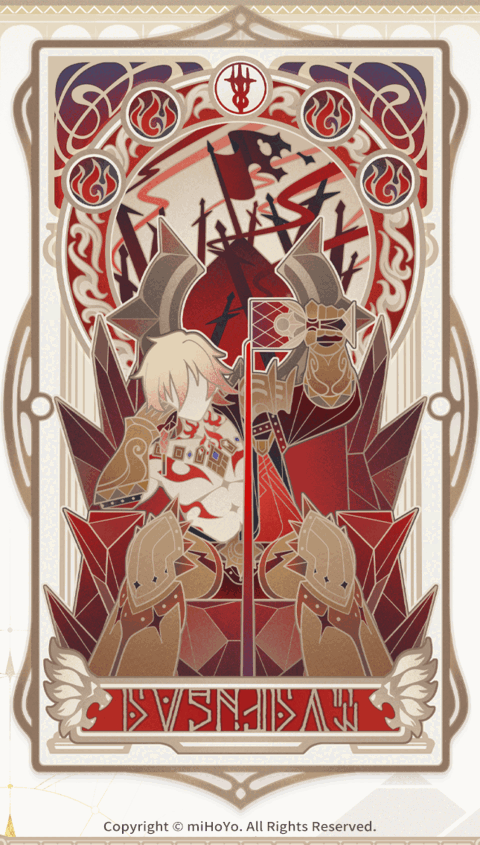
\includegraphics[width=0.22\textwidth]{assets/hsr_coreflame_icons/Icon_Coreflame_Strife.png}
\end{center}

矩阵变量的求导仍然处理同一个问题：当输入对象发生很小改变时，函数值的主要改变由什么决定。设输入变量为 \(X\in\mathbb{R}^{m\times n}\)，输入增量为 \(H\in\mathbb{R}^{m\times n}\)。若函数 \(F\) 在 \(X\) 附近有定义，则矩阵微积分首先关注 \(F(X+H)-F(X)\) 中关于 \(H\) 的线性主项。

矩阵空间 \(\mathbb{R}^{m\times n}\) 本身是一个有限维线性空间，微分概念可以直接迁移过来。若存在一个关于 \(H\) 的线性规则 \(\mathrm{D}F(X)\)，使得
\[
F(X+H)=F(X)+\mathrm{D}F(X)[H]+o(\|H\|),\qquad H\to 0,
\]
则称 \(F\) 在 \(X\) 处可微，并把 \(\mathrm{D}F(X)\) 称为 \(F\) 在 \(X\) 处的微分。这里的 \(\|H\|\) 可以取任意固定的矩阵范数；由于有限维空间中范数等价，判断余项是否为 \(o(\|H\|)\) 不依赖于某一种具体范数的本质选择。

后面反复出现“保留一阶项、丢掉高阶项”的判断，依赖几个简单的阶数规则。首先，有限维空间上的线性映射都是有界的。因此若 \(L\) 是关于矩阵增量 \(H\) 的线性规则，则存在常数 \(C\)，使得
\[
\|L[H]\|\le C\|H\|.
\]
线性主项总是 \(O(\|H\|)\)。

其次，固定矩阵左右乘不会改变增量的阶数。若 \(A\) 与 \(B\) 固定，则映射 \(H\mapsto AHB\) 仍是线性映射，所以存在常数 \(C\)，使得
\[
\|AHB\|\le C\|H\|.
\]
在常用的 Frobenius 范数或谱范数下，可以直接取类似 \(\|A\|\,\|H\|\,\|B\|\) 的上界；对任意固定矩阵范数，有限维范数等价保证同样的 \(O(\|H\|)\) 结论。

再次，两个增量相乘会产生二阶项。矩阵乘法是双线性映射，因此存在常数 \(C\)，使得
\[
\|HK\|\le C\|H\|\,\|K\|.
\]
特别地，若 \(K\) 与 \(H\) 同时趋于零，则 \(HK=O(\|H\|\,\|K\|)\)；若只用一个增量 \(H\)，则 \(H^2=O(\|H\|^2)\)。由于
\[
\frac{\|H\|^2}{\|H\|}=\|H\|\to0,
\]
所以 \(O(\|H\|^2)\) 项都属于 \(o(\|H\|)\)，可以归入一阶展开的余项。类似地，若某个量 \(R(H)=O(\|H\|)\)，则 \(H\,R(H)\) 或 \(R(H)\,H\) 都是 \(O(\|H\|^2)\)。

回到矩阵空间上的微分定义。这个定义中的关键对象仍然是 \(\mathrm{D}F(X)[H]\)。其中 \(H\) 是与 \(X\) 同型的矩阵增量，\(\mathrm{D}F(X)[H]\) 是函数增量的一阶主项，\(\mathrm{D}F(X)\) 本身则是从矩阵增量空间到输出空间的线性映射。若 \(F\) 是标量值函数，则 \(\mathrm{D}F(X)[H]\in\mathbb{R}\)；若 \(F\) 是矩阵值函数，则 \(\mathrm{D}F(X)[H]\) 与 \(F(X)\) 属于同一个输出矩阵空间。

为了把这个定义同熟悉的偏导数联系起来，可以暂时把矩阵元素视为坐标。令 \(E_{ij}\) 表示第 \((i,j)\) 个位置为 \(1\)、其余位置为 \(0\) 的标准矩阵，则任意增量 \(H=(h_{ij})\) 都可写成 \[H=\sum_{i,j}h_{ij}E_{ij}.\]
若 \(\mathrm{D}F(X)\) 是线性映射，则
\[
\mathrm{D}F(X)[H]=\sum_{i,j}h_{ij}\mathrm{D}F(X)[E_{ij}].
\]
当 \(F\) 是标量值函数时，\(\mathrm{D}F(X)[E_{ij}]\) 就是沿元素 \(x_{ij}\) 方向的一阶系数，也就是偏导数 \(\frac{\partial F}{\partial x_{ij}}(X)\)。因此，逐元素求偏导可以理解为逐个求出整体规则 \(H\mapsto \mathrm{D}F(X)[H]\) 在标准矩阵方向上的系数。

本章的例子只用于说明 Fréchet 展开如何工作，暂不系统讨论矩阵值函数。先考虑一个元素观测函数。固定指标 \(1\le i\le m\)、\(1\le j\le n\)，定义
\[
f_{ij}(X)=x_{ij}.
\]
当 \(X\) 变为 \(X+H\) 时，
\[
f_{ij}(X+H)-f_{ij}(X)=h_{ij}.
\]
因此
\[
Df_{ij}(X)[H]=h_{ij}.
\]
这个例子表明，元素偏导来自整体增量 \(H\) 在标准坐标方向上的分量，而不是独立于全微分之外的另一套规则。

再考虑标量线性测量。设 \(C,X,H\in\mathbb{R}^{m\times n}\)，定义
\[
\ell_C(X)=\sum_{i=1}^m\sum_{j=1}^n c_{ij}x_{ij}.
\]
则
\[
\ell_C(X+H)-\ell_C(X)
=\sum_{i=1}^m\sum_{j=1}^n c_{ij}h_{ij}.
\]
右端已经关于 \(H\) 线性，所以
\[
D\ell_C(X)[H]=\sum_{i=1}^m\sum_{j=1}^n c_{ij}h_{ij}.
\]
在这一层次上，只需要确认一阶主项是一个作用在矩阵增量上的线性规则；至于如何借助 Frobenius 内积把它写成梯度，将在下一章处理。

平方范数给出第一个非线性例子。设
\[
q(X)=\frac12\|X\|_F^2.
\]
直接展开可得
\[
q(X+H)-q(X)
=\frac12\|X+H\|_F^2-\frac12\|X\|_F^2.
\]
由 Frobenius 内积的双线性性，
\[
\frac12\|X+H\|_F^2-\frac12\|X\|_F^2
=\langle X,H\rangle_F+\frac12\|H\|_F^2.
\]
其中 \(\langle X,H\rangle_F\) 关于 \(H\) 线性，而 \(\frac12\|H\|_F^2=O(\|H\|_F^2)=o(\|H\|_F)\)。因此
\[
Dq(X)[H]=\langle X,H\rangle_F.
\]
这个例子展示了矩阵变量中的典型判断方式：完整增量中可能同时出现一阶项和二阶项，微分只保留关于输入增量的线性部分。

最后用双变量乘积说明阶数判断中的非交换性。设 \(X\in\mathbb{R}^{m\times n}\)、\(Y\in\mathbb{R}^{n\times p}\)，并令两个变量分别产生增量 \(H\in\mathbb{R}^{m\times n}\)、\(K\in\mathbb{R}^{n\times p}\)。对于 \(F(X,Y)=XY\)，有
\[
(X+H)(Y+K)-XY=HY+XK+HK.
\]
其中 \(HY\) 与 \(XK\) 关于 \((H,K)\) 线性，\(HK\) 是两个增量的乘积，属于二阶项。因此
\[
\mathrm{D}F(X,Y)[H,K]=HY+XK.
\]
用微分记号写作
\[
\mathrm{d}(XY)=(\mathrm{d}X)Y+X(\mathrm{d}Y).
\]
一般情形下，矩阵乘法不交换，且 \((\mathrm{d}X)Y\) 与 \(X(\mathrm{d}Y)\) 来自不同变量的增量。第七章将专门讨论输出为矩阵时，如何把这类一阶主项理解为从输入增量到输出增量的线性映射。

从上述例子可以提炼出矩阵变量求导的基本步骤。第一，明确哪些矩阵是变量，哪些矩阵是固定参数，并给变量增添同型增量。第二，展开 \(F(X+H)-F(X)\)，或者在多变量情形中展开 \(F(X+H,Y+K)-F(X,Y)\)。第三，保留关于增量的一阶项，把含有两个或更多增量因子的项归入余项。第四，把保留下来的线性部分记为 \(\mathrm{D}F(X)[H]\) 或 \(\mathrm{D}F(X,Y)[H,K]\)。

矩阵变量的微分就是作用在矩阵增量上的线性规则，元素偏导组成的矩阵只是这种规则在特定坐标下的表示。标量值矩阵函数中，\(\mathrm{D}F(X)[H]\) 是关于 \(H\) 的值为标量的线性映射；借助 Frobenius 内积，它可以进一步表示为矩阵梯度，这一点将在之后的章节中详细讨论。

\section{标量矩阵函数与 Frobenius 梯度}

\begin{center}
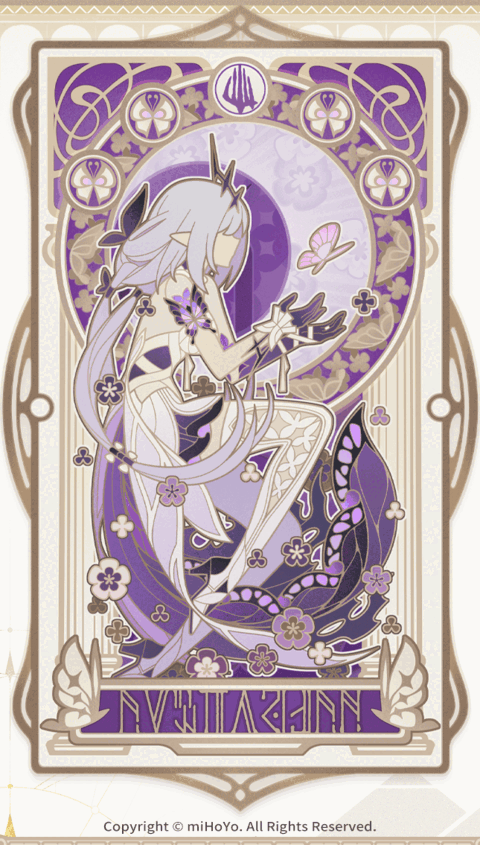
\includegraphics[width=0.22\textwidth]{assets/hsr_coreflame_icons/Icon_Coreflame_Death.png}
\end{center}

第三章中的矩阵变量函数可以有不同类型的输出；当输出是标量时，微分 \(\mathrm{D}f(X)[H]\) 是一个关于矩阵增量 \(H\) 的标量线性映射。由于 \(H\) 的每一个元素都可以独立变化，这个标量线性主项必然由各元素增量的系数共同决定；把这些系数重新排成与 \(X\) 同型的矩阵，就得到与向量梯度相对应的矩阵梯度。

在向量情形中，若 \(f:\mathbb{R}^n\to\mathbb{R}\) 可微，则 \(\mathrm{D}f(\bm{x})[\bm{u}]=\bm{\nabla} f(\bm{x})^\top \bm{u}\)。这里的 \(\bm{\nabla} f(\bm{x})\) 可以理解为线性主项中各个坐标增量的系数组成的向量，而内积 \(\bm{\nabla} f(\bm{x})^\top \bm{u}\) 则把“系数与增量逐项相乘再求和”写成紧凑形式。矩阵空间中的情形完全类似，只是坐标增量由 \(u_i\) 变成矩阵元素增量 \(h_{ij}\)；为了把对应的逐项求和写成矩阵形式，矩阵空间中采用 Frobenius 内积
\[
\langle A,B\rangle_F=\operatorname{tr}(A^\top B)=\sum_{i,j}a_{ij}b_{ij},
\]
其中 \(A,B\in\mathbb{R}^{m\times n}\)。该内积把同型矩阵的对应元素相乘后求和，因此正好适合记录标量线性主项中“系数矩阵与增量矩阵逐项配对”的结构。

设 \(L:\mathbb{R}^{m\times n}\to\mathbb{R}\) 是任意标量线性规则，令 \(E_{ij}\) 表示第 \((i,j)\) 个位置为 \(1\)、其余位置为 \(0\) 的标准矩阵。由于任意矩阵 \(H=(h_{ij})\) 都可写成 \[H=\sum_{i,j}h_{ij}E_{ij},\]
由线性性给出
\[
L(H)=\sum_{i,j}h_{ij}L(E_{ij}).
\]
\(L\) 完全由它在标准方向 \(E_{ij}\) 上的取值决定。把这些系数排成矩阵 \(G=(g_{ij})\)，其中 \(g_{ij}=L(E_{ij})\)，则
\[
L(H)=\sum_{i,j}g_{ij}h_{ij}=\langle G,H\rangle_F.
\]
若另有 \(G'\) 表示同一个线性规则，则对所有 \(H\) 有 \(\langle G-G',H\rangle_F=0\)，取 \(H=G-G'\) 得 \(G=G'\)。因此，矩阵到标量的线性主项总能唯一地写成某个同型矩阵与增量矩阵的 Frobenius 内积。

设 \(f:\mathbb{R}^{m\times n}\to\mathbb{R}\) 在 \(X\) 处可微。由上述坐标说明，存在唯一矩阵 \(G\in\mathbb{R}^{m\times n}\)，使得对任意同型增量 \(H\) 都有
\[
\mathrm{D}f(X)[H]=\langle G,H\rangle_F=\operatorname{tr}(G^\top H),
\]
这个唯一矩阵称为 \(f\) 在 \(X\) 处关于 Frobenius 内积的矩阵梯度，记为 \(\nabla_X f\)。换言之，矩阵梯度是把标量线性规则 \(H\mapsto \mathrm{D}f(X)[H]\) 写成 Frobenius 内积形式时出现的代表矩阵。

这个定义对应的基本书写格式为
\[
f(X+H)=f(X)+\langle \nabla_X f,H\rangle_F+o(\|H\|).
\]
若使用微分记号，并把矩阵增量写成 \(\mathrm{d}X\)，则同一关系写作
\[
\mathrm{d}f=\mathrm{D}f(X)[\mathrm{d}X]=\operatorname{tr}((\nabla_X f)^\top \mathrm{d}X).
\]
这里 \(\mathrm{d}f\) 是微分作用在实际增量 \(\mathrm{d}X\) 后得到的标量主项，\(\nabla_X f\) 是在 Frobenius 内积下表示该主项的矩阵。

先看最直接的线性标量函数。设 \(C\in\mathbb{R}^{m\times n}\)，定义
\[
f(X)=\langle C,X\rangle_F=\operatorname{tr}(C^\top X).
\]
则
\[
f(X+H)-f(X)=\langle C,X+H\rangle_F-\langle C,X\rangle_F=\langle C,H\rangle_F.
\]
因此 \(\mathrm{D}f(X)[H]=\langle C,H\rangle_F\)，并且 \(\nabla_X f=C\)。

Frobenius 范数平方保留了非线性标量函数中的同一结构。设
\[
f(X)=\frac12\|X\|_F^2=\frac12\langle X,X\rangle_F.
\]
当 \(X\) 变为 \(X+H\) 时，
\[
f(X+H)-f(X)=\frac12\langle X+H,X+H\rangle_F-\frac12\langle X,X\rangle_F
=\langle X,H\rangle_F+\frac12\langle H,H\rangle_F.
\]
最后一项为 \(O(\|H\|_F^2)\)，相对于 \(\|H\|_F\) 是高阶小量，所以
\[
\mathrm{D}f(X)[H]=\langle X,H\rangle_F,\qquad \nabla_X f=X.
\]
这里无需逐个展开所有元素也能确认梯度，因为一阶主项 \(H\mapsto \langle X,H\rangle_F\) 在 Frobenius 内积下的代表矩阵正是 \(X\)。

带中心的平方范数只改变基点处的一阶系数。设 \(B\in\mathbb{R}^{m\times n}\)，定义 \(f(X)=\frac12\|X-B\|_F^2\)。令 \(R=X-B\)，则
\[
f(X+H)-f(X)=\frac12\|R+H\|_F^2-\frac12\|R\|_F^2
=\langle R,H\rangle_F+\frac12\|H\|_F^2.
\]
因此
\[
\mathrm{D}f(X)[H]=\langle X-B,H\rangle_F,\qquad \nabla_X f=X-B.
\]
这个例子在最小二乘问题中会反复出现，其本质仍然是从增量展开中读出关于 \(H\) 的线性主项。

在第三章的坐标解释下，矩阵梯度与元素偏导的关系也很明确。若把 \(X\) 的所有元素 \(x_{ij}\) 都视为独立坐标，则标量函数 \(f(X)\) 的一阶展开具有形式
\[
f(X+H)-f(X)=\sum_{i,j}\frac{\partial f}{\partial x_{ij}}(X)\,h_{ij}+o(\|H\|).
\]
每一个偏导数都是线性主项在标准方向 \(E_{ij}\) 上的系数。另一方面，若已经把整体微分写成 \(\mathrm{D}f(X)[H]=\langle \nabla_X f,H\rangle_F\)，则沿前述标准矩阵 \(E_{ij}\) 方向的增量满足
\[
\mathrm{D}f(X)[E_{ij}]=\langle \nabla_X f,E_{ij}\rangle_F=(\nabla_X f)_{ij}.
\]
因此，在标准 Frobenius 内积下，
\[
(\nabla_X f)_{ij}=\frac{\partial f}{\partial x_{ij}}(X).
\]
这与前面由线性主项定义矩阵梯度的方式一致：逐坐标计算会逐个得到 \((\nabla_X f)_{ij}\)，而微分法先得到关于任意 \(H\) 的整体线性规则，再通过 Frobenius 内积读出同一个系数矩阵。微分法的优势不在于改变梯度的含义，而在于避免在复杂矩阵表达式中反复展开所有元素。

标量矩阵函数求导的步骤是：先通过增量展开得到 \(\mathrm{D}f(X)[H]\)，再用 Frobenius 内积把这个标量线性规则表示为 \(\langle \nabla_X f,H\rangle_F\)。较复杂的一阶主项通常还要整理成 \(\operatorname{tr}(G^\top H)\) 的形式，才能读出矩阵梯度，这一点将在下一章讨论。

\section{迹的循环性与梯度读取}

\begin{center}
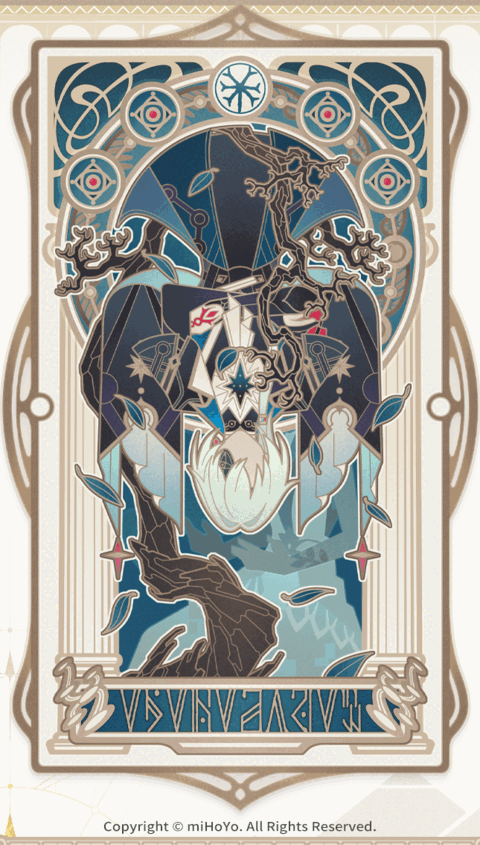
\includegraphics[width=0.22\textwidth]{assets/hsr_coreflame_icons/Icon_Coreflame_Reason.png}
\end{center}

第四章已经说明，标量矩阵函数的梯度由关系 \[\mathrm{D}f(X)[H]=\langle \nabla_X f,H\rangle_F = \operatorname{tr}((\nabla_X f)^\top H)\] 确定。实际计算时，先通过微分找到关于 \(H\) 的一阶主项，再利用迹的循环性把这个主项写成 \(\operatorname{tr}(G^\top H)\) 的形式；逐元素展开只是在特定坐标下的辅助方式。一旦这种形式成立，就有 \(\nabla_X f=G\)。

本章只使用几个直接服务于梯度读取的性质。首先，迹具有线性性，即 \[\operatorname{tr}(\alpha A+\beta B)=\alpha\operatorname{tr}(A)+\beta\operatorname{tr}(B),\]
其次，\(\operatorname{tr}(M)=\operatorname{tr}(M^\top)\)；再次，在乘积维度匹配时，迹具有循环性质，例如 \(\operatorname{tr}(ABC)=\operatorname{tr}(BCA)=\operatorname{tr}(CAB)\)。循环性质只允许整体循环移动因子，不能当作可交换乘法处理。

最简单的例子是迹线性函数。设 \(X\in\mathbb{R}^{m\times n}\)，\(A\in\mathbb{R}^{n\times m}\)，定义 \(f(X)=\operatorname{tr}(AX)\)。当 \(X\) 变为 \(X+H\) 时，
\[
f(X+H)-f(X)=\operatorname{tr}(A H).
\]
为了读出 Frobenius 梯度，需要把它写成 \(\operatorname{tr}(G^\top H)\)。由于 \(\operatorname{tr}(A H)=\operatorname{tr}((A^\top)^\top H)\)，可得
\[
\mathrm{D}f(X)[H]=\operatorname{tr}((A^\top)^\top H),\qquad \nabla_X f=A^\top.
\]
维度上，\(A^\top\in\mathbb{R}^{m\times n}\)，与变量 \(X\) 同型，因此能够与任意增量 \(H\) 作 Frobenius 内积。

含有左右乘因子的迹线性函数需要用到迹的循环性。设 \(X\in\mathbb{R}^{m\times n}\)、\(A\in\mathbb{R}^{p\times m}\)、\(B\in\mathbb{R}^{n\times p}\)，定义
\[
f(X)=\operatorname{tr}(A X B).
\]
则
\[
\mathrm{D}f(X)[H]=\operatorname{tr}(A H B).
\]
为了让 \(H\) 出现在 \(\operatorname{tr}(G^\top H)\) 中的最后一个位置，可以使用循环性质：
\[
\operatorname{tr}(A H B)=\operatorname{tr}(B A H)=\operatorname{tr}((A^\top B^\top)^\top H).
\]
因此 \(\nabla_X f=A^\top B^\top\)。这里的移动仅指迹内因子的循环移动，不能把 \(A\)、\(H\)、\(B\) 任意交换；若不借助迹的循环性质，直接把 \(H\) 当作可交换量移到末尾会导致错误。

迹二次型中会同时出现多个一阶项。设 \(X\in\mathbb{R}^{m\times n}\)，\(A\in\mathbb{R}^{m\times m}\)，定义 \(f(X)=\operatorname{tr}(X^\top A X)\)。由乘积微分规则得到
\[
\mathrm{d}f=\operatorname{tr}(\mathrm{d}X^\top A X)+\operatorname{tr}(X^\top A\,\mathrm{d}X).
\]
第一项满足 \(\operatorname{tr}(\mathrm{d}X^\top A X)=\operatorname{tr}((A X)^\top \mathrm{d}X)\)，第二项已经可写为 \(\operatorname{tr}((A^\top X)^\top \mathrm{d}X)\)。因此
\[
\mathrm{d}f=\operatorname{tr}(((A+A^\top)X)^\top \mathrm{d}X),
\]
从而
\[
\nabla_X f=(A+A^\top)X.
\]
若 \(A=A^\top\)，梯度才化为 \(2AX\)。没有对称性条件时，两个一阶项分别贡献 \(AX\) 与 \(A^\top X\)，不能直接合并为 \(2AX\)。

Frobenius 范数型目标是优化中最常见的例子。设 \(A\in\mathbb{R}^{p\times m}\)、\(X\in\mathbb{R}^{m\times n}\)、\(B\in\mathbb{R}^{p\times n}\)，定义
\[
f(X)=\frac12\|AX-B\|_F^2.
\]
记 \(R=AX-B\)，则当 \(X\) 的增量为 \(\mathrm{d}X\) 时，\(R\) 的增量为 \(A\,\mathrm{d}X\)，于是
\[
\mathrm{d}f=\langle R,A\,\mathrm{d}X\rangle_F=\operatorname{tr}(R^\top A\,\mathrm{d}X).
\]
利用迹的循环性与转置关系可得
\[
\operatorname{tr}(R^\top A\,\mathrm{d}X)=\operatorname{tr}((A^\top R)^\top \mathrm{d}X).
\]
因此
\[
\nabla_X f=A^\top(AX-B).
\]
这个推导中，微分法识别残差 \(R\) 与残差增量 \(A\,\mathrm{d}X\) 的一阶配对，迹的循环性把 \(\mathrm{d}X\) 的系数整理成与 \(X\) 同型的梯度矩阵。

这类计算通常按四步进行。第一，给变量 \(X\) 加上增量 \(\mathrm{d}X\)，只保留函数增量中的一阶项。第二，把标量一阶项写成迹表达式。第三，使用转置关系和迹的循环性，把表达式化为 \(\operatorname{tr}(G^\top \mathrm{d}X)\)。第四，根据 Frobenius 内积定义读出 \(\nabla_X f=G\)。最终读出的 \(G\) 必须与 \(X\) 同型，并且等式必须对任意同型增量 \(\mathrm{d}X\) 成立。

迹的循环性在这里的作用很具体：把标量一阶主项转换成 Frobenius 内积形式。线性函数、二次型、范数、逆矩阵和对数行列式的常用公式都可以按这个流程推导。

\section{一些矩阵函数的微分公式}

\begin{center}
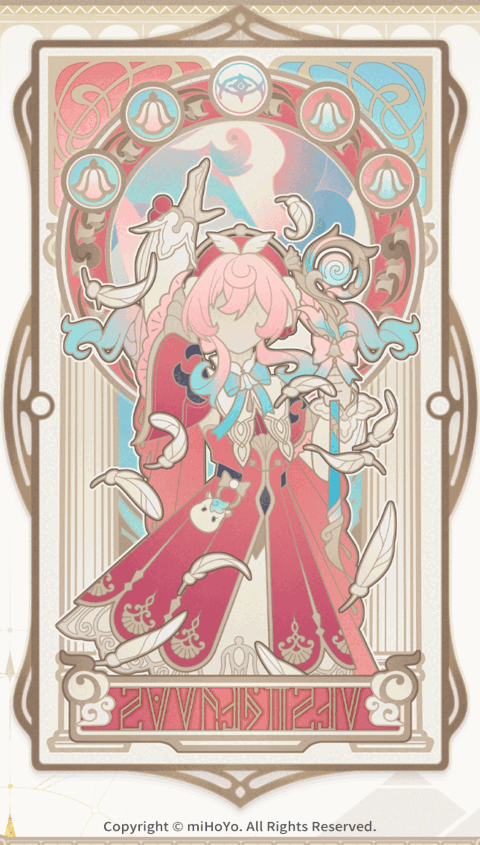
\includegraphics[width=0.22\textwidth]{assets/hsr_coreflame_icons/Icon_Coreflame_Sky.png}
\end{center}

前面已经说明，标量矩阵函数的梯度可以从一阶主项中读出。本章按函数类型整理常用公式；对已经完整计算过的例子只保留关键步骤，逆矩阵和对数行列式则展开推导。

对于迹线性函数，我们直接给出它们的梯度。设 \(X\in\mathbb{R}^{m\times n}\)，\(C\in\mathbb{R}^{m\times n}\)，若 \(f(X)=\langle C,X\rangle_F=\operatorname{tr}(C^\top X)\)，则
\[
\nabla_X f=C.
\]
若 \(f(X)=\operatorname{tr}(A X B)\)，其中 \(A\in\mathbb{R}^{p\times m}\)、\(B\in\mathbb{R}^{n\times p}\)，则
\[
\nabla_X f=A^\top B^\top.
\]
这类公式的共同点是：函数本身关于 \(X\) 已经线性，梯度就是与 \(\mathrm{d}X\) 配对的系数矩阵。

Frobenius 范数平方是最基本的二次型。设 \(B\in\mathbb{R}^{m\times n}\)，若 \(f(X)=\frac12\|X-B\|_F^2\)，则
\[
\nabla_X f=X-B.
\]
特别地，\(\nabla_X\frac12\|X\|_F^2=X\)。若带有左侧线性变换，
\[
f(X)=\frac12\|AX-B\|_F^2,
\]
其中 \(A\in\mathbb{R}^{p\times m}\)、\(X\in\mathbb{R}^{m\times n}\)、\(B\in\mathbb{R}^{p\times n}\)，则
\[
\nabla_X f=A^\top(AX-B).
\]
若线性变换在右侧，即 \(f(X)=\frac12\|XA-B\|_F^2\)，其中 \(A\in\mathbb{R}^{n\times q}\)、\(B\in\mathbb{R}^{m\times q}\)，则
\[
\nabla_X f=(XA-B)A^\top.
\]
左右乘的两个公式不同，原因是增量分别以 \(AH\) 和 \(HA\) 的形式进入残差，矩阵乘法顺序不能交换。

迹二次型也是前面已经推导过的核心例子。设 \(X\in\mathbb{R}^{m\times n}\)，\(A\in\mathbb{R}^{m\times m}\)，若 \(f(X)=\operatorname{tr}(X^\top A X)\)，则
\[
\nabla_X f=(A+A^\top)X.
\]
只有在 \(A=A^\top\) 时，公式才能简化为 \(\nabla_X f=2AX\)。

逆矩阵公式需要单独推导，因为它不能由多项式展开直接得到。设 \(X\in\mathbb{R}^{n\times n}\) 可逆，\(H\) 足够小时 \(X+H\) 也可逆。记
\[
\Delta=(X+H)^{-1}-X^{-1}.
\]
这里 \(\Delta\) 是逆矩阵输出的增量，目标是从 \(\Delta\) 中分离关于 \(H\) 的线性主项。由 \((X+H)(X+H)^{-1}=I\) 和 \(XX^{-1}=I\)，有
\[
(X+H)(X^{-1}+\Delta)-XX^{-1}=0.
\]
展开并消去 \(XX^{-1}\) 得
\[
X\Delta+HX^{-1}+H\Delta=0.
\]
若只保留一阶项，则乘积 \(H\Delta\) 暂时不参与主项，因为 \(\Delta\) 本身随 \(H\) 趋于零。于是线性主项 \(L\) 应满足
\[
XL+HX^{-1}=0,
\]
从而
\[
L=-X^{-1}HX^{-1}.
\]

还需要验证 \(H\Delta\) 确实只影响高阶余项。由上面的精确等式可得
\[
\Delta=-X^{-1}HX^{-1}-X^{-1}H\Delta.
\]
另一方面，由恒等式
\[
(X+H)^{-1}-X^{-1}=-X^{-1}H(X+H)^{-1}
\]
可知，\(\Delta\) 至少含有一个因子 \(H\)。当 \(H\) 足够小时，\(X+H\) 仍可逆，并且 \((X+H)^{-1}\) 在 \(X\) 的一个小邻域内有界；也就是说，存在常数 \(M\)，使得 \(\|(X+H)^{-1}\|\le M\)。于是
\[
\|\Delta\|
\le \|X^{-1}\|\,\|H\|\,\|(X+H)^{-1}\|
\le M\|X^{-1}\|\,\|H\|.
\]
这正是 \(\Delta=O(\|H\|)\) 的含义，即逆矩阵输出的增量与输入增量同阶。
于是 \(\|H\Delta\|=O(\|H\|^2)\)，从而 \(X^{-1}H\Delta=o(\|H\|)\)。代回 \(\Delta\) 的表达式，得到
\[
(X+H)^{-1}-X^{-1}=-X^{-1}HX^{-1}+o(\|H\|).
\]
因此
\[
\mathrm{D}(X^{-1})[H]=-X^{-1}HX^{-1}.
\]
这个公式要求基点 \(X\) 可逆，并且乘法顺序必须保留。

含逆矩阵的标量函数可由上一公式直接推出。设 \(A\in\mathbb{R}^{n\times n}\)，定义 \(f(X)=\operatorname{tr}(A X^{-1})\)，其中 \(X\) 可逆。由逆矩阵增量公式，
\[
f(X+H)-f(X)=\operatorname{tr}(A((X+H)^{-1}-X^{-1}))
=-\operatorname{tr}(A X^{-1}H X^{-1})+o(\|H\|).
\]
利用迹的循环性，
\[
-\operatorname{tr}(A X^{-1}H X^{-1})
=-\operatorname{tr}(X^{-1}A X^{-1}H)
=\operatorname{tr}((-X^{-\top}A^\top X^{-\top})^\top H).
\]
因此
\[
\nabla_X f=-X^{-\top}A^\top X^{-\top}.
\]
若 \(A\) 或 \(X\) 具有对称性，可以在这个公式的基础上进一步化简，但化简必须写明相应条件。

对数行列式的增量展开来自行列式乘法公式。设 \(X\in\mathbb{R}^{n\times n}\) 可逆，且 \(H\) 足够小时 \(X+H\) 与 \(X\) 位于同一个 \(\det\ne0\) 的连通区域内。由于
\[
\det(X+H)=\det X\cdot \det(I+X^{-1}H),
\]
有
\[
\log|\det(X+H)|-\log|\det X|=\log|\det(I+X^{-1}H)|.
\]
设 $E=(e_{ij})\in\mathbb{R}^{n\times n}$，记 $I+E=(\delta_{ij}+e_{ij})$，其中 $\delta_{ij}$ 为 Kronecker 符号。由行列式定义，

$$
\det(I+E)
=\sum_{\sigma\in S_n}\text{sgn}(\sigma)
\prod_{i=1}^n(\delta_{i,\sigma(i)}+e_{i,\sigma(i)}).
$$

先考虑恒等置换 $\sigma=\mathrm{id}$。此时

$$
\prod_{i=1}^n(1+e_{ii})
=1+\sum_{i=1}^n e_{ii}
+\sum_{1\le i<j\le n}e_{ii}e_{jj}
+\cdots
+e_{11}e_{22}\cdots e_{nn}.
$$

其中常数项为 $1$，一次项为 $\sum_{i=1}^n e_{ii}$，所有含两个或更多 $e_{ii}$ 的项都是 $O(\|E\|^2)$。

再考虑非恒等置换 $\sigma\ne\mathrm{id}$。若某个指标 $i$ 满足 $\sigma(i)\ne i$，则 $\delta_{i,\sigma(i)}=0$，对应因子只能取 $e_{i,\sigma(i)}$。由于置换不能只移动一个指标，非恒等置换至少存在两个指标 $i$ 使得 $\sigma(i)\ne i$。因此每个非恒等置换对应的乘积至少含有两个 $E$ 的元素，从而整体为 $O(\|E\|^2)$。

于是 $\det(I+E)$ 的常数项与一次项完全由恒等置换贡献，得到
\[
\det(I+E)=1+\sum_i e_{ii}+O(\|E\|^2)=1+\operatorname{tr}(E)+O(\|E\|^2).
\]
再由一元展开 \(\log(1+s)=s+O(s^2)\) 得到
\[
\log|\det(I+E)|=\operatorname{tr}(E)+o(\|E\|).
\]
取 \(E=X^{-1}H\) 得
\[
\log|\det(X+H)|-\log|\det X|
=\operatorname{tr}(X^{-1}H)+o(\|H\|)
=\operatorname{tr}((X^{-\top})^\top H)+o(\|H\|).
\]
因此
\[
\nabla_X \log|\det X|=X^{-\top}.
\]
在对称正定矩阵空间中，\(\log\det X\) 是实值函数，且 \(X^{-\top}=X^{-1}\)，所以普通矩阵空间中的梯度表达化为 \(X^{-1}\)。若变量还受到对称约束，后文需要进一步讨论可行增量与梯度投影。

这些公式可以直接复用，但适用条件必须同时保留，尤其是可逆性、正定性、对称性和维度匹配。当输出不再是标量时，导数本身应保留为从输入增量到输出增量主项的线性映射，而不一定能读成一个梯度矩阵。

\section{矩阵值函数的导数}

\begin{center}
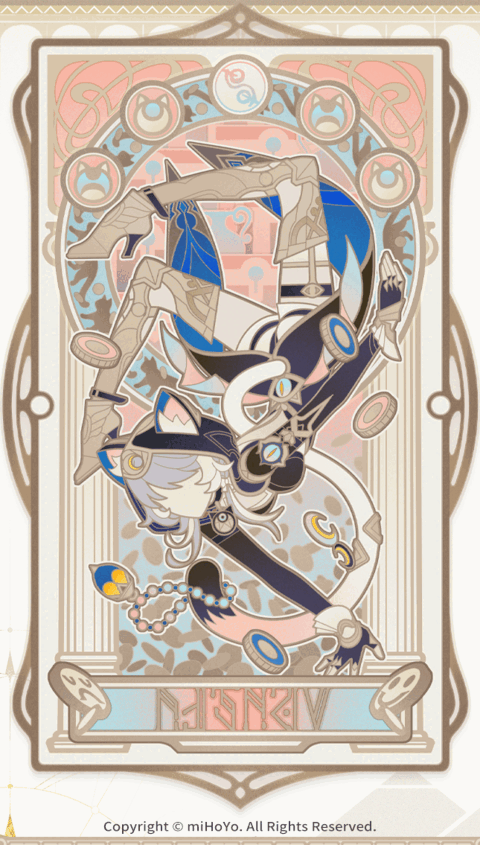
\includegraphics[width=0.22\textwidth]{assets/hsr_coreflame_icons/Icon_Coreflame_Trickery.png}
\end{center}

标量值矩阵函数的一阶主项 \(\mathrm{D}f(X)[H]\) 是标量，可以借助 Frobenius 内积表示为矩阵梯度。若函数的输出本身也是矩阵，一阶主项也位于输出矩阵空间中。矩阵值函数的导数首先应被理解为从输入增量到输出增量主项的线性映射。

设 \(F:\mathbb{R}^{m\times n}\to\mathbb{R}^{p\times q}\)，若在 \(X\) 处存在关于 \(H\in\mathbb{R}^{m\times n}\) 的线性规则 \(\mathrm{D}F(X)\)，使得
\[
F(X+H)=F(X)+\mathrm{D}F(X)[H]+o(\|H\|),
\]
则 \(\mathrm{D}F(X)[H]\in\mathbb{R}^{p\times q}\)。这里的 \(\mathrm{D}F(X)\) 是把输入矩阵增量 \(H\) 变成输出矩阵主项的规则，一般不能理解为一个与 \(X\) 同型的矩阵。只有在输出是标量时，才需要进一步用内积代表这个规则并得到梯度。

恒等映射给出最简单的例子。设 \(F(X)=X\)，其中 \(X,H\in\mathbb{R}^{m\times n}\)。由于
\[
F(X+H)-F(X)=H,
\]
可得
\[
\mathrm{D}F(X)[H]=H.
\]
这个导数把输入增量原样送到输出增量，不需要读出梯度；若强行寻找一个“梯度矩阵”，反而会遮蔽导数作为映射的本质。

固定矩阵左乘和右乘是最常用的线性映射。设 \(A\in\mathbb{R}^{p\times m}\)、\(B\in\mathbb{R}^{n\times q}\)，定义
\[
F(X)=A X B,\qquad X\in\mathbb{R}^{m\times n}.
\]
则
\[
F(X+H)-F(X)=A H B.
\]
因此
\[
\mathrm{D}F(X)[H]=A H B.
\]
这个公式中的导数与基点 \(X\) 无关，因为 \(F\) 本身就是线性映射。维度上，\(H\in\mathbb{R}^{m\times n}\)，而 \(AHB\in\mathbb{R}^{p\times q}\)，正好属于输出空间。

转置映射表明导数可以改变矩阵形状。设 \(F(X)=X^\top\)，其中 \(X\in\mathbb{R}^{m\times n}\)。则
\[
F(X+H)-F(X)=H^\top,
\]
所以
\[
\mathrm{D}F(X)[H]=H^\top.
\]
这里输入增量属于 \(\mathbb{R}^{m\times n}\)，输出主项属于 \(\mathbb{R}^{n\times m}\)。

非线性矩阵值函数中，一阶主项通常依赖于基点。考虑 \(F(X)=X^\top X\)，其中 \(X\in\mathbb{R}^{m\times n}\)，输出属于 \(\mathbb{R}^{n\times n}\)。当 \(X\) 变为 \(X+H\) 时，
\[
F(X+H)-F(X)=(X+H)^\top(X+H)-X^\top X
=H^\top X+X^\top H+H^\top H.
\]
最后一项是二阶小量，因此
\[
\mathrm{D}F(X)[H]=H^\top X+X^\top H.
\]
该表达式关于 \(H\) 线性，但系数依赖于基点 \(X\)。同时，输出矩阵是对称矩阵，因为 \(H^\top X+X^\top H\) 等于其自身的转置，这与 \(X^\top X\) 的输出结构一致。

另一个常见例子是 \(F(X)=XX^\top\)，其中 \(X\in\mathbb{R}^{m\times n}\)，输出属于 \(\mathbb{R}^{m\times m}\)。展开可得
\[
(X+H)(X+H)^\top-XX^\top=H X^\top+XH^\top+HH^\top,
\]
从而
\[
\mathrm{D}F(X)[H]=H X^\top+XH^\top.
\]
这个例子与 \(X^\top X\) 只有乘法顺序的差别，但输出空间和导数形式都不同，不能把两者混为同一个公式。

逆矩阵作为矩阵值函数的导数已经在第六章中出现。设 \(X\in\mathbb{R}^{n\times n}\) 可逆，\(F(X)=X^{-1}\)，则
\[
F(X+H)-F(X)=-X^{-1}H X^{-1}+o(\|H\|),
\]
因此
\[
\mathrm{D}F(X)[H]=-X^{-1}H X^{-1}.
\]
这里 \(\mathrm{D}F(X)\) 把输入增量 \(H\) 左右各乘一个固定矩阵 \(-X^{-1}\) 和 \(X^{-1}\)，仍然是关于 \(H\) 的线性映射。可逆性是该公式的基本条件，乘法顺序也不能改变。

矩阵值函数同样满足链式法则，但链式法则应按线性映射的复合来理解。设 \(G:\mathbb{R}^{m\times n}\to\mathbb{R}^{r\times s}\)，\(F:\mathbb{R}^{r\times s}\to\mathbb{R}^{p\times q}\)，并令 \(Y=G(X)\)。若二者均可微，则
\[
\mathrm{D}(F\circ G)(X)[H]=\mathrm{D}F(Y)[\mathrm{D}G(X)[H]].
\]
先由 \(G\) 把输入增量 \(H\) 送到输出增量主项 \(\mathrm{D}G(X)[H]\)，再由 \(F\) 的导数把这个矩阵主项送到最终输出的一阶主项。这个公式的关键在于两个线性规则的连续作用，矩阵相乘只是具体表示中可能出现的形式。

一个简单复合例子展示了这种写法。设 \(G(X)=AXB\)，\(F(Y)=Y^\top Y\)。由前面的公式，\(\mathrm{D}G(X)[H]=AHB\)，而
\[
\mathrm{D}F(Y)[K]=K^\top Y+Y^\top K.
\]
因此
\[
\mathrm{D}(F\circ G)(X)[H]=(AHB)^\top(AXB)+(AXB)^\top(AHB).
\]
整个表达式仍然关于 \(H\) 线性，并且输出属于与 \(Y^\top Y\) 相同的矩阵空间。

矩阵值函数也可以坐标化，但坐标化不构成导数的定义。若把输入矩阵和输出矩阵都按元素排成向量，线性映射 \(H\mapsto \mathrm{D}F(X)[H]\) 可以表示为一个普通矩阵乘法；这个普通矩阵就是向量化坐标下的 Jacobian。坐标表示会用到向量化和 Kronecker 积，但在概念上，矩阵值函数的导数仍是作用在矩阵增量上的线性映射，不能与标量函数情形中的梯度矩阵混同。

\section{向量化与 Kronecker 积}

\begin{center}
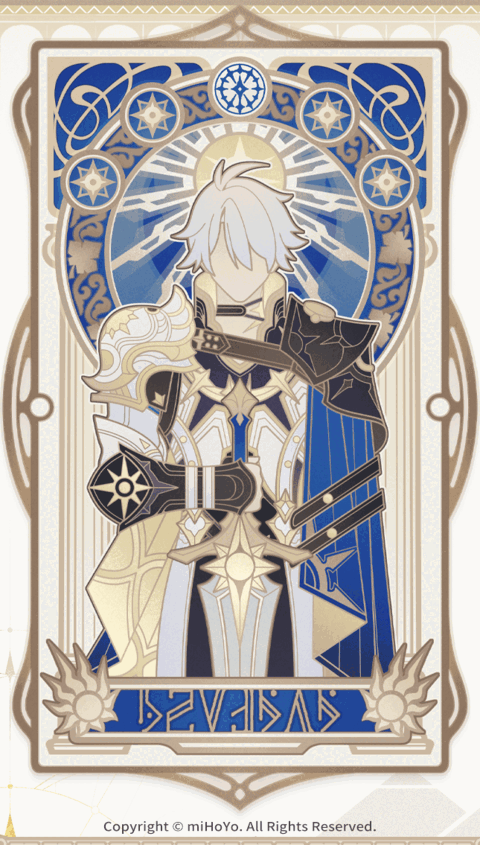
\includegraphics[width=0.22\textwidth]{assets/hsr_coreflame_icons/Icon_Coreflame_Worldbearing.png}
\end{center}

矩阵值函数的导数本身是线性映射 \(H\mapsto \mathrm{D}F(X)[H]\)。为了把这种线性映射交给普通矩阵代数处理，可以把输入矩阵和输出矩阵按固定顺序排成向量。这样得到的矩阵就可以看作导数在选定坐标下的表示。

本章采用列堆叠的向量化约定。若 \(X=[\bm{x}_1,\ldots,\bm{x}_n]\in\mathbb{R}^{m\times n}\)，其中 \(\bm{x}_j\in\mathbb{R}^m\) 是第 \(j\) 列，则
\[
\operatorname{vec}(X)=
\begin{bmatrix}
x_1\\
\vdots\\
x_n
\end{bmatrix}\in\mathbb{R}^{mn}.
\]
因此，矩阵增量 \(H\in\mathbb{R}^{m\times n}\) 可以用 \(\operatorname{vec}(H)\in\mathbb{R}^{mn}\) 表示；若输出 \(\mathrm{D}F(X)[H]\in\mathbb{R}^{p\times q}\)，则它的坐标表示为 \(\operatorname{vec}(\mathrm{D}F(X)[H])\in\mathbb{R}^{pq}\)。

第二章已经在向量值函数中引入过 Jacobian 矩阵；这里使用同一个观念，只是先把矩阵输入和矩阵输出都向量化。设 \(\bm{z}=\operatorname{vec}(X)\)，并把 \(F(X)\) 的输出写成 \(\operatorname{vec}(F(X))\)。若存在矩阵 \(J\in\mathbb{R}^{pq\times mn}\)，使得对任意增量 \(H\) 都有
\[
\operatorname{vec}(F(X+H))=\operatorname{vec}(F(X))+J\,\operatorname{vec}(H)+o(\|H\|),
\]
则这个矩阵 \(J\) 称为 \(F\) 在 \(X\) 处的 Jacobian 矩阵，或者说是导数 \(\mathrm{D}F(X)\) 在列堆叠坐标下的矩阵表示。等价地，
\[
\operatorname{vec}(\mathrm{D}F(X)[H])=J\,\operatorname{vec}(H).
\]
因此，Jacobian 矩阵是把线性映射 \(\mathrm{D}F(X)\) 写进固定坐标后的系数矩阵。

Kronecker 积用于描述“左右乘”这类矩阵线性映射的坐标矩阵。若 \(B=(b_{ij})\in\mathbb{R}^{r\times s}\)，\(A\in\mathbb{R}^{p\times q}\)，则
\[
B\otimes A=
\begin{bmatrix}
b_{11}A&\cdots&b_{1s}A\\
\vdots&\ddots&\vdots\\
b_{r1}A&\cdots&b_{rs}A
\end{bmatrix}\in\mathbb{R}^{pr\times qs}.
\]
这个定义把 \(B\) 的每个元素替换成对应倍数的 \(A\)，其主要用途是在向量化后记录矩阵乘法对列的线性组合。

核心恒等式是
\[
\operatorname{vec}(A H B)=(B^\top\otimes A)\operatorname{vec}(H),
\]
其中 \(A\in\mathbb{R}^{p\times m}\)、\(H\in\mathbb{R}^{m\times n}\)、\(B\in\mathbb{R}^{n\times q}\)。维度上，\(\operatorname{vec}(H)\in\mathbb{R}^{mn}\)，\(\operatorname{vec}(AHB)\in\mathbb{R}^{pq}\)，而 \(B^\top\otimes A\in\mathbb{R}^{pq\times mn}\)，因此该矩阵正好把输入增量的坐标送到输出增量的坐标。

这个恒等式可由列结构直接推出。设 \(B=[b_1,\ldots,b_q]\)，则 \(AHB\) 的第 \(j\) 列为 \(AHb_j\)。若 \(b_j=(b_{1j},\ldots,b_{nj})^\top\)，则 \(Hb_j=\sum_k b_{kj}h_k\)，其中 \(h_k\) 是 \(H\) 的第 \(k\) 列；因此
\[
AHb_j=\sum_k b_{kj}A h_k.
\]
把所有列按顺序堆叠后，得到的系数矩阵正是由 \(B^\top\) 的元素作为块系数、以 \(A\) 为块组成的 \(B^\top\otimes A\)。

由此可以把第七章中的线性映射 \(H\mapsto AHB\) 写成普通矩阵乘法。若 \(F(X)=AXB\)，则 \(\mathrm{D}F(X)[H]=AHB\)，于是
\[
\operatorname{vec}(\mathrm{D}F(X)[H])=(B^\top\otimes A)\operatorname{vec}(H).
\]
因此，在向量化坐标下，\(F\) 的 Jacobian 矩阵就是 \(B^\top\otimes A\)。这里的 Jacobian 依赖于列堆叠约定；若改变向量化顺序，坐标矩阵也会随之改变，但线性映射 \(H\mapsto AHB\) 本身不变。

转置映射的导数也可以坐标化。对于 \(F(X)=X^\top\)，导数为 \(\mathrm{D}F(X)[H]=H^\top\)。回忆导数是一个线性映射，则在列堆叠后，存在一个只由维度决定的置换矩阵 \(K_{m,n}\)，使得
\[
\operatorname{vec}(H^\top)=K_{m,n}\operatorname{vec}(H).
\]
于是转置映射的 Jacobian 是 \(K_{m,n}\)。有些矩阵值函数的坐标表示需要由重排坐标的置换矩阵刻画，不能只依赖普通左右乘形式。

非线性矩阵值函数的 Jacobian 通常依赖于基点。以 \(F(X)=X^\top X\) 为例，第七章已经得到
\[
\mathrm{D}F(X)[H]=H^\top X+X^\top H.
\]
为了得到 Jacobian，需要分别把 \(H\mapsto H^\top X\) 和 \(H\mapsto X^\top H\) 坐标化。第一项需要先用置换矩阵表示转置，再用 Kronecker 积表示右乘 \(X\)；第二项则直接对应左乘 \(X^\top\)。因此 Jacobian 的具体矩阵由置换矩阵和 Kronecker 积组合而成。重要的是，坐标矩阵虽然形式较长，但其来源仍然是清楚的一阶主项 \(H^\top X+X^\top H\)。

对于标量值函数，也可以使用向量化表示梯度。若 \(f:\mathbb{R}^{m\times n}\to\mathbb{R}\)，并且 \(\nabla_X f=G\)，则
\[
\mathrm{D}f(X)[H]=\langle G,H\rangle_F=\operatorname{vec}(G)^\top\operatorname{vec}(H).
\]
因此，若把 \(f\) 视为普通函数 \(\tilde f(\operatorname{vec}X)\)，其向量梯度就是 \(\operatorname{vec}(\nabla_X f)\)。矩阵梯度与向量化梯度并不矛盾；前者保留矩阵形状，后者是同一对象在列堆叠坐标下的表示。

向量化和 Kronecker 积的作用可以概括为：把矩阵增量之间的线性规则坐标化。它们适合用于需要显式 Jacobian 矩阵的场合，例如数值实现、线性方程求解或二阶公式推导；但在推导一阶主项时，直接保留 \(H\mapsto \mathrm{D}F(X)[H]\) 往往更简洁。二阶展开与 Hessian 中也会遇到同样的选择：先保留线性映射，需要坐标矩阵时再向量化。

\section{二阶微分与 Hessian}

\begin{center}
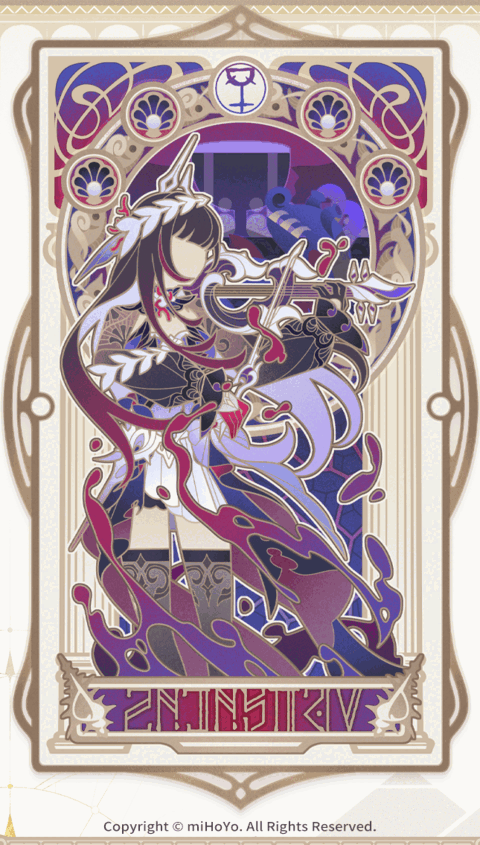
\includegraphics[width=0.22\textwidth]{assets/hsr_coreflame_icons/Icon_Coreflame_Ocean.png}
\end{center}

一阶微分描述函数增量中的线性主项，二阶展开则刻画这一主项随基点变化的方式。对于标量函数，二阶项对应局部曲率；在优化问题中，它决定驻点附近的上凸、下凸或鞍点行为。Hessian 可以理解为梯度或一阶微分的再次变化。

在向量变量情形中，设 \(f:\mathbb{R}^n\to\mathbb{R}\) 二阶可微。若 \(\bm{x}\) 的增量为 \(\bm{u}\)，则一阶展开为
\[
f(\bm{x}+\bm{u})=f(\bm{x})+\bm{\nabla} f(\bm{x})^\top \bm{u}+o(\|\bm{u}\|).
\]
若继续保留二阶主项，则有
\[
f(\bm{x}+\bm{u})=f(\bm{x})+\bm{\nabla} f(\bm{x})^\top \bm{u}+\frac12 \bm{u}^\top \nabla^2 f(\bm{x})\bm{u}+o(\|\bm{u}\|^2).
\]
其中 \(\nabla^2 f(\bm{x})\in\mathbb{R}^{n\times n}\) 称为 Hessian 矩阵，它描述梯度 \(\bm{\nabla} f(\bm{x})\) 对输入变化的一阶响应。

从梯度增量看，若 \(\bm{\nabla} f:\mathbb{R}^n\to\mathbb{R}^n\) 可微，则
\[
\bm{\nabla} f(\bm{x}+\bm{u})=\bm{\nabla} f(\bm{x})+\nabla^2 f(\bm{x})\bm{u}+o(\|\bm{u}\|).
\]
因此 Hessian 是梯度映射的 Jacobian。它先描述梯度如何变化，再由这种变化产生二阶曲率项，从而间接刻画函数增量中的二阶部分。

一元函数 \(f(x)=x^2\) 是一个最简单的例子。由于 \(f'(x)=2x\)、\(f''(x)=2\)，有
\[
f(x+h)=f(x)+2xh+\frac12\cdot 2h^2.
\]
多元二次型 \(f(\bm{x})=\bm{x}^\top A\bm{x}\) 展示了同样结构。前面已经得到 \(\bm{\nabla} f(\bm{x})=(A+A^\top)\bm{x}\)，因此
\[
\nabla^2 f(\bm{x})=A+A^\top.
\]
若 \(A=A^\top\)，则 Hessian 为 \(2A\)。这里对称性仍然是简化的必要条件；没有对称性时，二阶项由 \(A+A^\top\) 决定，不能直接写成 \(2A\)。

矩阵变量中的二阶展开保持同一形式，只是输入增量变为矩阵。设 \(f:\mathbb{R}^{m\times n}\to\mathbb{R}\)，若在 \(X\) 处二阶可微，则
\[
f(X+H)=f(X)+\mathrm{D}f(X)[H]+\frac12 \mathrm{D}^2 f(X)[H,H]+o(\|H\|^2).
\]
这里 \(\mathrm{D}^2 f(X)\) 是作用在两个矩阵增量上的双线性映射，而 \(\mathrm{D}^2 f(X)[H,H]\) 是把两个位置都取为同一个增量 \(H\) 后得到的二阶主项。二阶微分的输出仍是标量，但与一阶微分不同，它依赖于两个增量方向。

若采用 Frobenius 内积表示一阶微分，且 \(\nabla_X f\) 可微，则 Hessian 也可以理解为梯度映射的导数。具体地，
\[
\nabla_X f(X+H)=\nabla_X f(X)+\mathcal{H}_X[H]+o(\|H\|),
\]
其中 \(\mathcal{H}_X\) 是把矩阵增量 \(H\) 送到梯度增量主项的线性映射。于是二阶项可以写成
\[
\frac12 \mathrm{D}^2 f(X)[H,H]= \frac12 \langle H,\mathcal{H}_X[H]\rangle_F.
\]
矩阵变量中的 Hessian 最自然的形式是从矩阵增量到矩阵增量的线性映射；四维数组只是进一步坐标化后的表示。

Frobenius 范数平方是最简单的矩阵例子。设
\[
f(X)=\frac12\|X-B\|_F^2.
\]
第四章已经得到 \(\nabla_X f=X-B\)。因此当 \(X\) 变为 \(X+H\) 时，梯度增量为
\[
\nabla_X f(X+H)-\nabla_X f(X)=H.
\]
所以 Hessian 映射为 \(\mathcal{H}_X[H]=H\)，并且
\[
f(X+H)=f(X)+\langle X-B,H\rangle_F+\frac12\langle H,H\rangle_F.
\]
这里的二阶项正是 \(\frac12\|H\|_F^2\)，说明该函数在所有方向上的曲率相同。

带左乘的最小二乘目标展示了非平凡的 Hessian。设
\[
f(X)=\frac12\|AX-B\|_F^2,
\]
其中 \(A\in\mathbb{R}^{p\times m}\)。由 \(\nabla_X f=A^\top(AX-B)\) 可知，当 \(X\) 增加 \(H\) 时，
\[
\nabla_X f(X+H)-\nabla_X f(X)=A^\top A H.
\]
因此 Hessian 映射为
\[
\mathcal{H}_X[H]=A^\top A H.
\]
对应的二阶项为
\[
\frac12\langle H,A^\top A H\rangle_F=\frac12\|AH\|_F^2.
\]
曲率由 \(A^\top A\) 决定；若 \(A\) 的某些方向被压缩，目标函数在相应方向上的二阶变化也会减弱。

若需要显式 Hessian 矩阵，可以使用第八章的向量化坐标。令 \(\bm{h}=\operatorname{vec}(H)\)。对于 \(f(X)=\frac12\|AX-B\|_F^2\)，由于 \(\mathcal{H}_X[H]=A^\top A H\)，有
\[
\operatorname{vec}(\mathcal{H}_X[H])=(I_n\otimes A^\top A)\bm{h}.
\]
因此在列堆叠坐标下，Hessian 矩阵为 \(I_n\otimes A^\top A\)。这个矩阵是 Hessian 映射 \(\mathcal{H}_X\) 的坐标表示。

Hessian 与优化条件直接相关。若 \(\bm{x}_\ast\) 是无约束局部极小点，通常需要 \(\bm{\nabla} f(\bm{x}_\ast)=\bm{0}\)，并且 Hessian 在该点半正定，即 \(\bm{u}^\top\nabla^2 f(\bm{x}_\ast)\bm{u}\ge0\) 对所有方向 \(\bm{u}\) 成立。矩阵变量中，对应条件是
\[
\langle H,\mathcal{H}_{X_\ast}[H]\rangle_F\ge0
\]
对所有矩阵增量 \(H\) 成立。若该二次型在所有非零方向上为正，则驻点附近具有严格的二阶增长；若存在方向使其为负，则沿该方向会出现二阶下降。

Hessian 描述一阶微分或梯度的再次变化，二阶项是 Hessian 作用在增量后形成的二次型。向量化可以把 Hessian 映射写成普通矩阵，但二阶结构本身仍然来自 \(f(X+H)\) 中关于 \(H\) 的二阶主项。若变量受到约束，允许的增量不再是全部矩阵方向，梯度和 Hessian 条件也必须沿可行方向理解。

\section{约束变量与可行增量}

\begin{center}
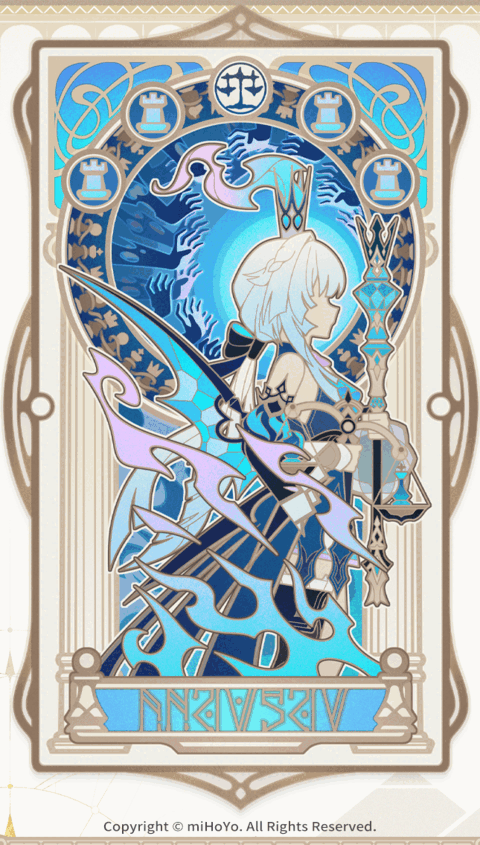
\includegraphics[width=0.22\textwidth]{assets/hsr_coreflame_icons/Icon_Coreflame_Law.png}
\end{center}

无约束情形中，矩阵变量可以沿任意方向变化，一阶条件可以对所有增量 \(H\) 检验。受约束问题的差别在于，变量只能留在某个集合中，允许的增量不再是整个矩阵空间。此时微分主项仍然是核心对象，但它只需要在可行方向上满足相应条件。

设变量 \(X\) 被限制在集合 \(\mathcal{M}\) 中。若从 \(X\) 出发的一条可行曲线 \(X(t)\in\mathcal{M}\) 满足 \(X(0)=X\)，则 \(H=X'(0)\) 表示 \(X\) 处的一个可行增量。所有这种一阶可行增量构成的空间称为切空间，记为 \(T_X\mathcal{M}\)。对于标量函数 \(f\)，若 \(X\) 是约束下的局部极小点，则对所有 \(H\in T_X\mathcal{M}\) 都应有
\[
\mathrm{D}f(X)[H]=0.
\]
若采用 Frobenius 内积表示 \(\mathrm{D}f(X)[H]=\langle \nabla_X f,H\rangle_F\)，则一阶条件变为
\[
\langle \nabla_X f,H\rangle_F=0,\qquad H\in T_X\mathcal{M}.
\]
普通梯度不必为零；它只需要与所有可行方向正交。

最简单的约束是对称矩阵空间。若变量满足 \(X=X^\top\)，则可行增量也必须满足
\[
H=H^\top.
\]
因此切空间就是所有对称矩阵组成的线性空间。对于一般矩阵空间中的梯度 \(G=\nabla_X f\)，真正影响对称可行方向的一阶项是
\[
\langle G,H\rangle_F=\left\langle \frac{G+G^\top}{2},H\right\rangle_F,\qquad H=H^\top.
\]
因此，在对称矩阵变量上，欧氏梯度应投影为
\[
\operatorname{sym}(G)=\frac{G+G^\top}{2}.
\]
约束极小点的一阶条件是 \(\operatorname{sym}(\nabla_X f)=0\)，不能直接使用一般矩阵意义下的 \(\nabla_X f=0\)。

正定矩阵集合 \(\mathbb{S}_{++}^n\) 是对称矩阵空间中的开集。若 \(X\in\mathbb{S}_{++}^n\)，则足够小的对称增量 \(H=H^\top\) 会使 \(X+H\) 仍位于正定集合内，因此其切空间仍是所有对称矩阵。正定性本身影响函数定义域和可行区域，例如 \(\log\det X\) 只在正定矩阵上自然成为实值函数；但在内部点处，一阶可行方向仍由对称性决定。

以 \(f(X)=-\log\det X+\operatorname{tr}(CX)\) 为例，其中 \(X\in\mathbb{S}_{++}^n\)，\(C=C^\top\)。在一般矩阵空间中，\(\nabla_X(-\log\det X)=-X^{-\top}\)，而正定约束下 \(X^{-\top}=X^{-1}\)。又由于 \(C\) 对称，梯度为
\[
\nabla_X f=-X^{-1}+C.
\]
该梯度已经位于对称矩阵空间中，因此一阶条件为 \(-X^{-1}+C=0\)。若目标中的普通梯度不是对称矩阵，则必须先取对称部分，再在对称方向上判断驻点条件。

正交约束中，“允许的增量不再任意”这一点更明显。设 \(X\in\mathbb{R}^{n\times p}\) 满足
\[
X^\top X=I_p.
\]
若 \(X(t)^\top X(t)=I_p\) 且 \(X(0)=X\)、\(X'(0)=H\)，对约束取一阶变化得
\[
H^\top X+X^\top H=0.
\]
因此切空间为
\[
T_X\mathcal{M}=\{H\in\mathbb{R}^{n\times p}:X^\top H+H^\top X=0\}.
\]
对于约束优化，驻点条件应写成切空间上的正交条件：
\[
\langle \nabla_X f,H\rangle_F=0,\qquad H\in T_X\mathcal{M}.
\]

这个条件可以写成投影形式。给定普通梯度 \(G=\nabla_X f\)，它在正交约束切空间上的投影为
\[
\operatorname{Proj}_{T_X}(G)=G-X\,\operatorname{sym}(X^\top G),
\]
其中 \(\operatorname{sym}(M)=\frac12(M+M^\top)\)。因此正交约束下的一阶驻点条件可以写为
\[
G-X\,\operatorname{sym}(X^\top G)=0.
\]
等价地，\(G\) 的切向分量必须为零，普通梯度只能指向约束集合的法向方向。

当 \(p=n\) 且 \(X\) 是正交矩阵时，切空间还可以写成
\[
T_X O(n)=\{X\Omega:\Omega^\top=-\Omega\}.
\]
这是因为 \(X^\top H\) 必须是反对称矩阵。此时一阶条件 \(\langle G,X\Omega\rangle_F=0\) 对所有反对称 \(\Omega\) 成立，等价于 \(X^\top G\) 是对称矩阵。这个形式常用于正交矩阵优化，因为它直接把可行方向写成“当前点乘反对称增量”。

约束情形下的二阶条件也必须沿可行方向理解。若 \(X_\ast\) 是约束局部极小点，首先需要一阶主项在所有切向方向上消失；其次，二阶主项应在可行方向上非负。对于线性约束空间，例如对称矩阵空间，这可以直接写为
\[
\mathrm{D}^2 f(X_\ast)[H,H]\ge0,\qquad H\in T_{X_\ast}\mathcal{M}.
\]
对于曲面型约束，例如正交约束，二阶可行曲线还会带来约束曲率项；完整二阶条件需要结合拉格朗日函数处理。这里要保留的判断是：二阶分析不能沿所有矩阵方向进行，而必须沿可行方向进行。

约束不改变微分的基本定义，但会改变允许代入微分的增量集合。无约束问题要求一阶主项对所有 \(H\) 消失；约束问题只要求它对所有 \(H\in T_X\mathcal{M}\) 消失。梯度投影、对称化和正交切空间条件，都是这一原则在不同约束集合中的具体形式。

\section{典型优化问题中的统一方法}

\begin{center}
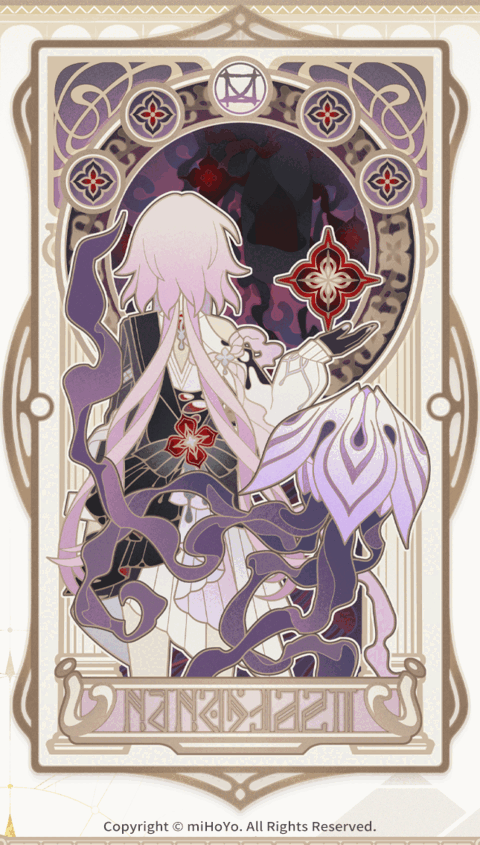
\includegraphics[width=0.22\textwidth]{assets/hsr_coreflame_icons/Icon_Coreflame_Time.png}
\end{center}

矩阵微积分在优化中的作用，是把目标函数在当前点附近的主要变化写成关于增量的线性主项，并由此得到一阶条件。无约束问题要求这个线性主项对所有增量消失；约束问题要求它对所有可行增量消失。微分、梯度、Hessian 和投影公式都服务于这个判断。

最小二乘问题是最基本的例子。设 \(A\in\mathbb{R}^{p\times m}\)、\(B\in\mathbb{R}^{p\times n}\)，考虑
\[
f(X)=\frac12\|AX-B\|_F^2,\qquad X\in\mathbb{R}^{m\times n}.
\]
第六章已经得到
\[
\nabla_X f=A^\top(AX-B).
\]
无约束一阶条件为
\[
A^\top(AX-B)=0,
\]
即
\[
A^\top A X=A^\top B.
\]
这就是矩阵形式的正规方程。若 \(A^\top A\) 可逆，则唯一驻点为 \(X=(A^\top A)^{-1}A^\top B\)；若 \(A^\top A\) 不可逆，一阶条件仍然描述所有最小二乘解所在的仿射集合。

正则化最小二乘只是在一阶条件中增加一个稳定项。设 \(\lambda>0\)，
\[
f(X)=\frac12\|AX-B\|_F^2+\frac{\lambda}{2}\|X\|_F^2.
\]
由梯度的线性性，
\[
\nabla_X f=A^\top(AX-B)+\lambda X.
\]
一阶条件为
\[
(A^\top A+\lambda I_m)X=A^\top B.
\]
由于 \(A^\top A+\lambda I_m\) 正定，该方程有唯一解。这里的正则化项改变了 Hessian 映射，从 \(H\mapsto A^\top A H\) 变为 \(H\mapsto (A^\top A+\lambda I_m)H\)，从而消除了 \(A^\top A\) 可能存在的零曲率方向。

带右乘的二次优化对乘法顺序更敏感。若
\[
f(X)=\frac12\|XA-B\|_F^2+\frac{\lambda}{2}\|X\|_F^2,
\]
其中 \(A\in\mathbb{R}^{n\times q}\)、\(B\in\mathbb{R}^{m\times q}\)，则
\[
\nabla_X f=(XA-B)A^\top+\lambda X.
\]
一阶条件为
\[
X(AA^\top+\lambda I_n)=BA^\top.
\]
这个方程与左乘情形不同，未知矩阵 \(X\) 位于系数矩阵的左侧；直接套用左乘公式会破坏矩阵乘法顺序。

对数行列式目标展示了正定约束中的一阶条件。设 \(C=C^\top\)，考虑
\[
f(X)=-\log\det X+\operatorname{tr}(CX),\qquad X\in\mathbb{S}_{++}^n.
\]
由于 \(\nabla_X(-\log\det X)=-X^{-1}\)，且 \(\nabla_X\operatorname{tr}(CX)=C\)，可得
\[
\nabla_X f=-X^{-1}+C.
\]
正定集合是对称矩阵空间中的开集，因此内部驻点满足
\[
-X^{-1}+C=0.
\]
若 \(C\) 正定，则解为 \(X=C^{-1}\)。若 \(C\) 不是正定矩阵，则该方程无法在 \(\mathbb{S}_{++}^n\) 中产生可行解，目标函数的极小性需要重新结合定义域和边界行为分析。

另一类常见问题是带有迹逆矩阵项的目标。设 \(A=A^\top\succeq0\)，考虑
\[
f(X)=\operatorname{tr}(A X^{-1})+\operatorname{tr}(CX),\qquad X\in\mathbb{S}_{++}^n,
\]
其中 \(C=C^\top\)。一般公式为 \(\nabla_X\operatorname{tr}(A X^{-1})=-X^{-\top}A^\top X^{-\top}\)。在正定对称约束下，这化为
\[
\nabla_X f=-X^{-1}AX^{-1}+C.
\]
因此内部一阶条件为
\[
X^{-1}AX^{-1}=C.
\]
这个方程虽非普通线性方程，但仍然来自同一个微分主项；后续求解可以使用矩阵方程、特征分解或数值迭代，而一阶条件本身由梯度直接确定。

正交约束问题展示了投影条件的作用。设 \(X\in\mathbb{R}^{n\times p}\) 满足 \(X^\top X=I_p\)，考虑线性目标
\[
f(X)=-\operatorname{tr}(C^\top X).
\]
普通欧氏梯度为 \(G=-C\)。约束驻点条件应写成切向投影为零：
\[
G-X\operatorname{sym}(X^\top G)=0.
\]
代入 \(G=-C\)，可得
\[
C=X\operatorname{sym}(X^\top C).
\]
该条件蕴含 \(X^\top C\) 是对称矩阵，同时还要求 \(C\) 落在由 \(X\) 的列空间决定的法向结构中；对于矩形 Stiefel 约束，不能只用 \(X^\top C\) 对称替代完整的投影方程。在线性目标下，普通梯度一般不会消失；约束极值只要求目标的一阶变化在所有正交可行方向上消失。

若 \(X\in O(n)\) 是方阵正交矩阵，切空间可写为 \(H=X\Omega\)，其中 \(\Omega^\top=-\Omega\)。对于同一个目标 \(f(X)=-\operatorname{tr}(C^\top X)\)，一阶变化为
\[
\mathrm{D}f(X)[X\Omega]=-\operatorname{tr}(C^\top X\Omega).
\]
该式对所有反对称 \(\Omega\) 消失，当且仅当 \(X^\top C\) 是对称矩阵。这与投影条件一致，但切空间表达更直接地显示了可行方向的结构。

矩阵优化的一阶分析可以固定为一个流程。第一，明确变量所在空间以及允许的增量；第二，写出目标函数的一阶主项或调用已经推导出的梯度公式；第三，无约束问题令普通梯度为零，约束问题令梯度在切空间上的投影为零；第四，再根据 Hessian 或二阶主项判断驻点的局部性质。

这里的重点不是增加新的求导公式，而是把已有工具合并为一种方法。最小二乘使用 Frobenius 范数梯度，对数行列式使用逆矩阵和行列式微分，正交约束使用切空间与投影；这些类型不同的问题，都通过“输入增量如何决定目标函数变化”联系起来。

\section{总结}

\begin{center}
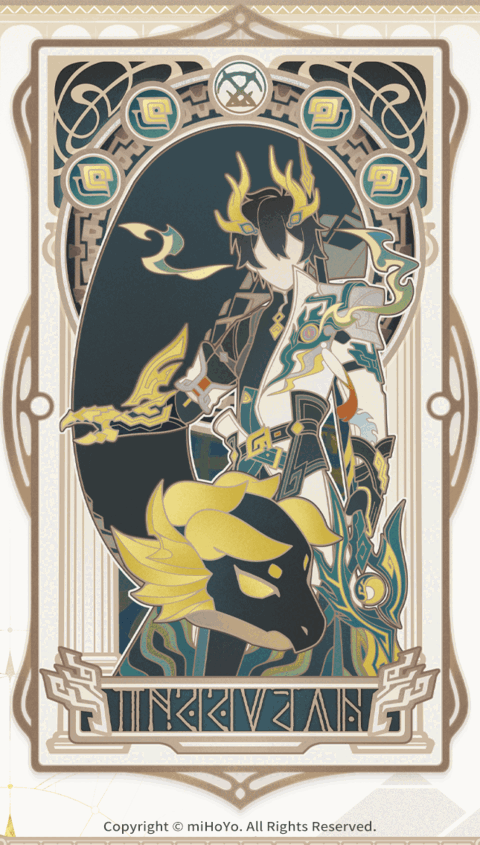
\includegraphics[width=0.22\textwidth]{assets/hsr_coreflame_icons/Icon_Coreflame_Earth.png}
\end{center}

矩阵微积分反复处理同一个问题：输入发生小变化时，函数值的主要变化由什么决定。若干求导公式只有放回这一问题中，才不再是互不相关的记忆对象。无论输入是实数、向量还是矩阵，基本形式都可以写成
\[
F(X+H)=F(X)+\mathrm{D}F(X)[H]+o(\|H\|).
\]
其中 \(H\) 是输入增量，\(\mathrm{D}F(X)[H]\) 是函数增量的一阶主项，\(\mathrm{D}F(X)\) 是把输入增量送到一阶主项的线性规则。所有后续概念都围绕这个线性规则展开。

微分是这里最基本的对象。对于标量值函数，微分输出一个数；对于矩阵值函数，微分输出一个矩阵。它的共同含义始终是：在基点 \(X\) 附近，函数增量最先由哪个关于 \(H\) 的线性规则控制。逐元素偏导、方向导数和 Jacobian 矩阵都可以理解为这个线性规则的不同坐标表达，不能视为与微分平行的另一套概念。

梯度只出现在标量值函数中。若 \(f:\mathbb{R}^{m\times n}\to\mathbb{R}\)，则 \(\mathrm{D}f(X)[H]\) 是矩阵增量 \(H\) 上的标量线性规则。采用 Frobenius 内积后，存在唯一矩阵 \(\nabla_X f\)，使得
\[
\mathrm{D}f(X)[H]=\langle \nabla_X f,H\rangle_F=\operatorname{tr}((\nabla_X f)^\top H).
\]
因此，梯度是微分在选定内积下的代表矩阵，而微分这条线性规则本身不依赖于这种代表形式。改变内积约定会改变代表对象，但不会改变微分这条线性规则。

迹的循环性服务于梯度读取。许多标量矩阵函数的一阶主项先以 \(\operatorname{tr}(AHB)\)、\(\operatorname{tr}(X^\top A H)\) 或类似形式出现；利用迹的循环性和转置关系，可以把它化成 \(\operatorname{tr}(G^\top H)\)，从而读出 \(\nabla_X f=G\)。迹的作用在于把一阶主项转换为 Frobenius 内积形式，而不应脱离微分过程成为独立技巧。

矩阵值函数的导数应保持为线性映射。若 \(F:\mathbb{R}^{m\times n}\to\mathbb{R}^{p\times q}\)，则
\[
\mathrm{D}F(X)[H]\in\mathbb{R}^{p\times q}.
\]
例如 \(F(X)=AXB\) 的导数是 \(H\mapsto AHB\)，\(F(X)=X^\top X\) 的导数是 \(H\mapsto H^\top X+X^\top H\)。这些表达保留了输入空间、输出空间和矩阵乘法顺序，是导数最自然的形式。

Jacobian 矩阵、向量化和 Kronecker 积属于坐标化工具。若把矩阵按列堆叠成向量，则线性映射 \(H\mapsto \mathrm{D}F(X)[H]\) 可以写成
\[
\operatorname{vec}(\mathrm{D}F(X)[H])=J\,\operatorname{vec}(H).
\]
这个 \(J\) 是导数在列堆叠坐标下的 Jacobian 矩阵。特别地，恒等式
\[
\operatorname{vec}(AHB)=(B^\top\otimes A)\operatorname{vec}(H)
\]
表明 \(H\mapsto AHB\) 的坐标矩阵是 \(B^\top\otimes A\)。因此，Kronecker 积的作用是把矩阵间线性规则写成普通矩阵乘法，并不引入新的微分规则。

Hessian 描述二阶主项。对于标量函数，一阶微分刻画局部线性变化，Hessian 刻画这个线性映射如何随基点继续变化。向量变量中，二阶展开为
\[
f(\bm{x}+\bm{u})=f(\bm{x})+\bm{\nabla} f(\bm{x})^\top \bm{u}+\frac12\bm{u}^\top\nabla^2 f(\bm{x})\bm{u}+o(\|\bm{u}\|^2).
\]
矩阵变量中，对应形式为
\[
f(X+H)=f(X)+\mathrm{D}f(X)[H]+\frac12 \mathrm{D}^2 f(X)[H,H]+o(\|H\|^2).
\]
若用梯度映射描述 Hessian，则 \(\nabla_X f(X+H)=\nabla_X f(X)+\mathcal{H}_X[H]+o(\|H\|)\)，二阶项为 \(\langle H,\mathcal{H}_X[H]\rangle_F\)。Hessian 既可以理解为二阶双线性映射，也可以理解为梯度变化的线性映射。

约束投影来自可行增量的限制。无约束问题中，局部极小点的一阶条件要求 \(\mathrm{D}f(X)[H]=0\) 对所有 \(H\) 成立，因此普通梯度为零。受约束问题中，允许的增量只属于切空间 \(T_X\mathcal{M}\)，一阶条件变为
\[
\mathrm{D}f(X)[H]=0,\qquad H\in T_X\mathcal{M}.
\]
于是普通梯度不必为零，只需其切向分量为零。对称矩阵约束产生对称化投影，正交约束产生 \(G-X\operatorname{sym}(X^\top G)\) 这样的切空间投影；这些公式都来自同一个事实：只有可行方向上的一阶变化才与约束极值有关。

对称矩阵变量还容易引起另一类记号差异。设 \(X=X^\top\)，且某个标量函数在对称空间中的 Frobenius 梯度为 \(G=G^\top\)，即对所有对称增量 \(H=H^\top\) 有
\[
\mathrm{D}f(X)[H]=\langle G,H\rangle_F.
\]
若改用上三角元素 \(x_{ij}\ (i\le j)\) 作为独立坐标，则
\[
\langle G,H\rangle_F
=\sum_i G_{ii}H_{ii}+2\sum_{i<j}G_{ij}H_{ij}.
\]
因此，上三角独立坐标下的偏导数组在非对角元处会多出一个因子 \(2\)。若把这组坐标偏导重新排成对称矩阵，得到的矩阵为
\[
G_{\mathrm{coord}}=2G-\operatorname{diag}(G).
\]
反过来，从 \(G_{\mathrm{coord}}\) 回到 Frobenius 梯度时，对角元保持不变，非对角元除以 \(2\)。例如 \(f(X)=\log\det X\) 在 \(X\succ0\) 上的 Frobenius 梯度是 \(X^{-1}\)，而上三角独立坐标偏导矩阵是
\[
2X^{-1}-\operatorname{diag}(X^{-1}).
\]
两种写法表示的是同一个微分线性规则，只是坐标和内积约定不同。

常用公式表也应按这一结构理解。线性函数、Frobenius 范数、最小二乘、迹二次型、逆矩阵和对数行列式都不宜孤立记忆。每个公式都来自三步：写出函数增量，保留关于输入增量的线性主项，再根据输出类型选择表示方式。标量值函数读出梯度，矩阵值函数保留线性映射，需要坐标时再向量化。

这些联系也解释了常见错误的来源。把矩阵乘法当作可交换乘法，会破坏一阶主项中的因子顺序；在没有说明内积时直接读出梯度，会混淆微分和代表矩阵；对对称或正交变量直接使用普通梯度条件，会忽略可行增量并不任意；把 Jacobian 当作导数本身，则会忘记它依赖具体坐标约定。

最终，矩阵微积分可以被理解为有限维线性空间上的微分语言。微分负责找到输入增量到函数增量主项的线性规则；梯度是在内积下表示标量线性规则的对象；迹的循环性帮助把标量主项写成 Frobenius 内积；向量化和 Kronecker 积把矩阵线性映射坐标化；Hessian 描述二阶曲率；约束投影把一阶和二阶条件限制到可行方向。掌握这些位置之后，矩阵求导的关键就从公式表记忆转向增量中的线性主项识别，以及相应表示方式的选择。

\section{常见矩阵微积分公式表}

\begin{center}
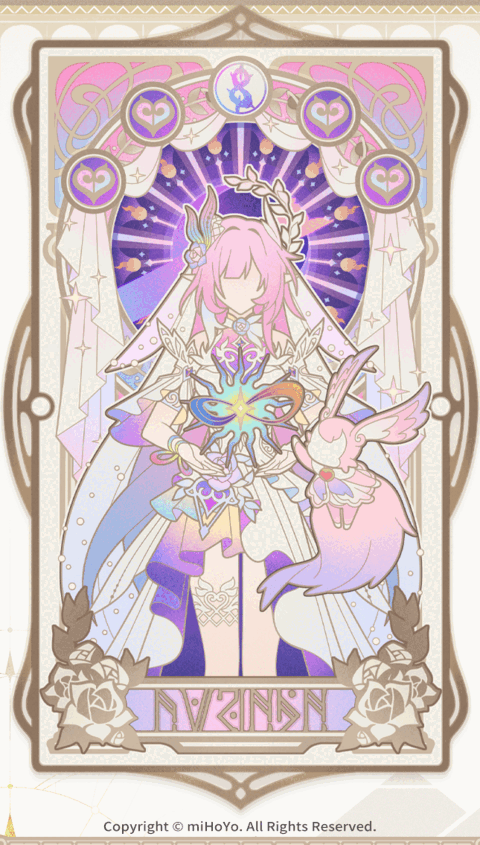
\includegraphics[width=0.22\textwidth]{assets/hsr_coreflame_icons/Icon_Coreflame_Genesis.png}
\end{center}

下面把常见例子汇总成公式表。表中的梯度默认采用 Frobenius 内积，即
\[
\mathrm{D}f(X)[H]=\operatorname{tr}((\nabla_X f)^\top H).
\]
若变量带有对称、正定或正交约束，表中会单独标明普通梯度、可行增量和投影条件，避免把无约束公式直接套用到受约束问题中。

\subsection{无约束标量值函数}

\begingroup
\scriptsize
\[
\begin{array}{c|c|c|c}
\hline
f(X) & \text{Condition} & \mathrm{D}f(X)[H] & \nabla_X f \\
\hline
\langle C,X\rangle_F=\operatorname{tr}(C^\top X)
& -
& \operatorname{tr}(C^\top H)
& C \\
\hline
\operatorname{tr}(AXB)
& -
& \operatorname{tr}(AHB)
& A^\top B^\top  \\
\hline
\det X
& \det X\ne 0
& \det(X)\operatorname{tr}(X^{-1}H)
& \det(X)X^{-\top} \\
\hline
\det(AXB)
& \det(AXB)\ne 0
& \det(AXB)\operatorname{tr}((AXB)^{-1}AHB)
& \det(AXB)A^\top(AXB)^{-\top}B^\top \\
\hline
\log\det(AXB)
& \det(AXB)>0
& \operatorname{tr}((AXB)^{-1}AHB)
& A^\top(AXB)^{-\top}B^\top \\
\hline
\frac{1}{2}\|X-B\|_F^2
& -
& \langle X-B,H\rangle_F
& X-B \\
\hline
\frac{1}{2}\|AX-B\|_F^2
& -
& \langle AX-B,AH\rangle_F
& A^\top(AX-B) \\
\hline
\frac{1}{2}\|XA-B\|_F^2
& -
& \langle XA-B,HA\rangle_F
& (XA-B)A^\top \\
\hline
\operatorname{tr}(X^\top AX)
& -
& \operatorname{tr}(H^\top AX)+\operatorname{tr}(X^\top AH)
& (A+A^\top)X \\
\hline
\operatorname{tr}(XAX^\top)
& -
& \operatorname{tr}(HAX^\top)+\operatorname{tr}(XAH^\top)
& X(A+A^\top) \\
\hline
\operatorname{tr}(X^\top AXB)
& -
& \operatorname{tr}(H^\top AXB)+\operatorname{tr}(X^\top AHB)
& AXB+A^\top XB^\top \\
\hline
\log\det(X^\top AX)
& A=A^\top,\ \det(X^\top AX)>0
& \operatorname{tr}((X^\top AX)^{-1}(H^\top AX+X^\top AH))
& 2AX(X^\top AX)^{-1} \\
\hline
\operatorname{tr}(AX^{-1})
& \det X\ne 0
& -\operatorname{tr}(AX^{-1}HX^{-1})
& -X^{-\top}A^{\top}X^{-\top} \\
\hline
\log|\det X|
& \det X\ne 0
& \operatorname{tr}(X^{-1}H)
& X^{-\top} \\
\hline
-\log\det X+\operatorname{tr}(CX)
& X\succ 0,\ C=C^\top
& \operatorname{tr}\bigl((-X^{-1}+C)H\bigr),\ H=H^\top
& -X^{-1}+C \\
\hline
\end{array}
\]
\endgroup

上述公式的使用方式相同：先确定变量 \(X\) 和增量 \(H\)，再确认一阶主项是否已经写成 Frobenius 内积形式。特别地，\(\operatorname{tr}(X^\top A X)\) 只有在 \(A=A^\top\) 时梯度才化为 \(2AX\)。

\subsection{矩阵值函数与线性映射}

\[
\begin{array}{c|c|c|c}
\hline
F(X) & \text{Condition} & \mathrm{D}F(X)[H] & \text{Vectorized Coordinate Representation} \\
\hline
X
& -
& H
& \operatorname{vec}(H) \\
\hline
AXB
& -
& AHB
& (B^\top \otimes A)\operatorname{vec}(H) \\
\hline
X^\top
& -
& H^\top
& K_{m,n}\operatorname{vec}(H) \\
\hline
X^\top X
& \text{无}
& H^\top X+X^\top H
& - \\
\hline
XX^\top
& -
& HX^\top+XH^\top
& - \\
\hline
X^{-1}
& \det X\ne 0
& -X^{-1}HX^{-1}
& -(X^{-\top}\otimes X^{-1})\operatorname{vec}(H) \\
\hline
\end{array}
\]

矩阵值函数的导数应优先理解为 \(H\mapsto \mathrm{D}F(X)[H]\) 的线性映射。向量化坐标表示只是在需要显式 Jacobian 矩阵时使用；例如 \(H\mapsto AHB\) 的坐标矩阵是 \(B^\top\otimes A\)，但导数本身仍然是左右乘规则。

\subsection{二阶信息}

\[
\begin{array}{c|c|c}
\hline
f(X)
& \mathcal{H}_X[H]
& \frac{1}{2} \mathrm{D}^2 f(X)[H,H] \\
\hline
\frac{1}{2}\|X-B\|_F^2
& H
& \frac{1}{2}\|H\|_F^2 \\
\hline
\frac{1}{2}\|AX-B\|_F^2
& A^\top AH
& \frac{1}{2}\|AH\|_F^2 \\
\hline
\frac{1}{2}\|XA-B\|_F^2
& HAA^{\mathrm T}
& \frac{1}{2}\|HA\|_F^2 \\
\hline
\operatorname{tr}(X^\top AX)
& (A+A^{\mathrm T})H
& \frac{1}{2}\langle H,(A+A^\top)H\rangle_F \\
\hline
\end{array}
\]

Hessian 表中的 \(\mathcal{H}_X[H]\) 是梯度增量的一阶主项，本身可以保留为作用在 \(H\) 上的线性映射。若需要坐标矩阵，可以再对 \(H\) 向量化；例如 \(H\mapsto A^\top A H\) 的坐标矩阵是 \(I_n\otimes A^\top A\)。

这些表格应作为推导结果的索引使用，不能替代推导。每个公式在使用前都需要检查三件事：变量所在空间是否正确，矩阵乘法是否匹配，是否存在对称、正定、\(\det X\ne0\) 或正交等附加条件。只要这些条件明确，表中的公式都可以回到同一个来源，即函数增量中关于输入增量的线性主项。


\clearpage
\thispagestyle{empty}
\vspace*{\fill}
\begin{center}
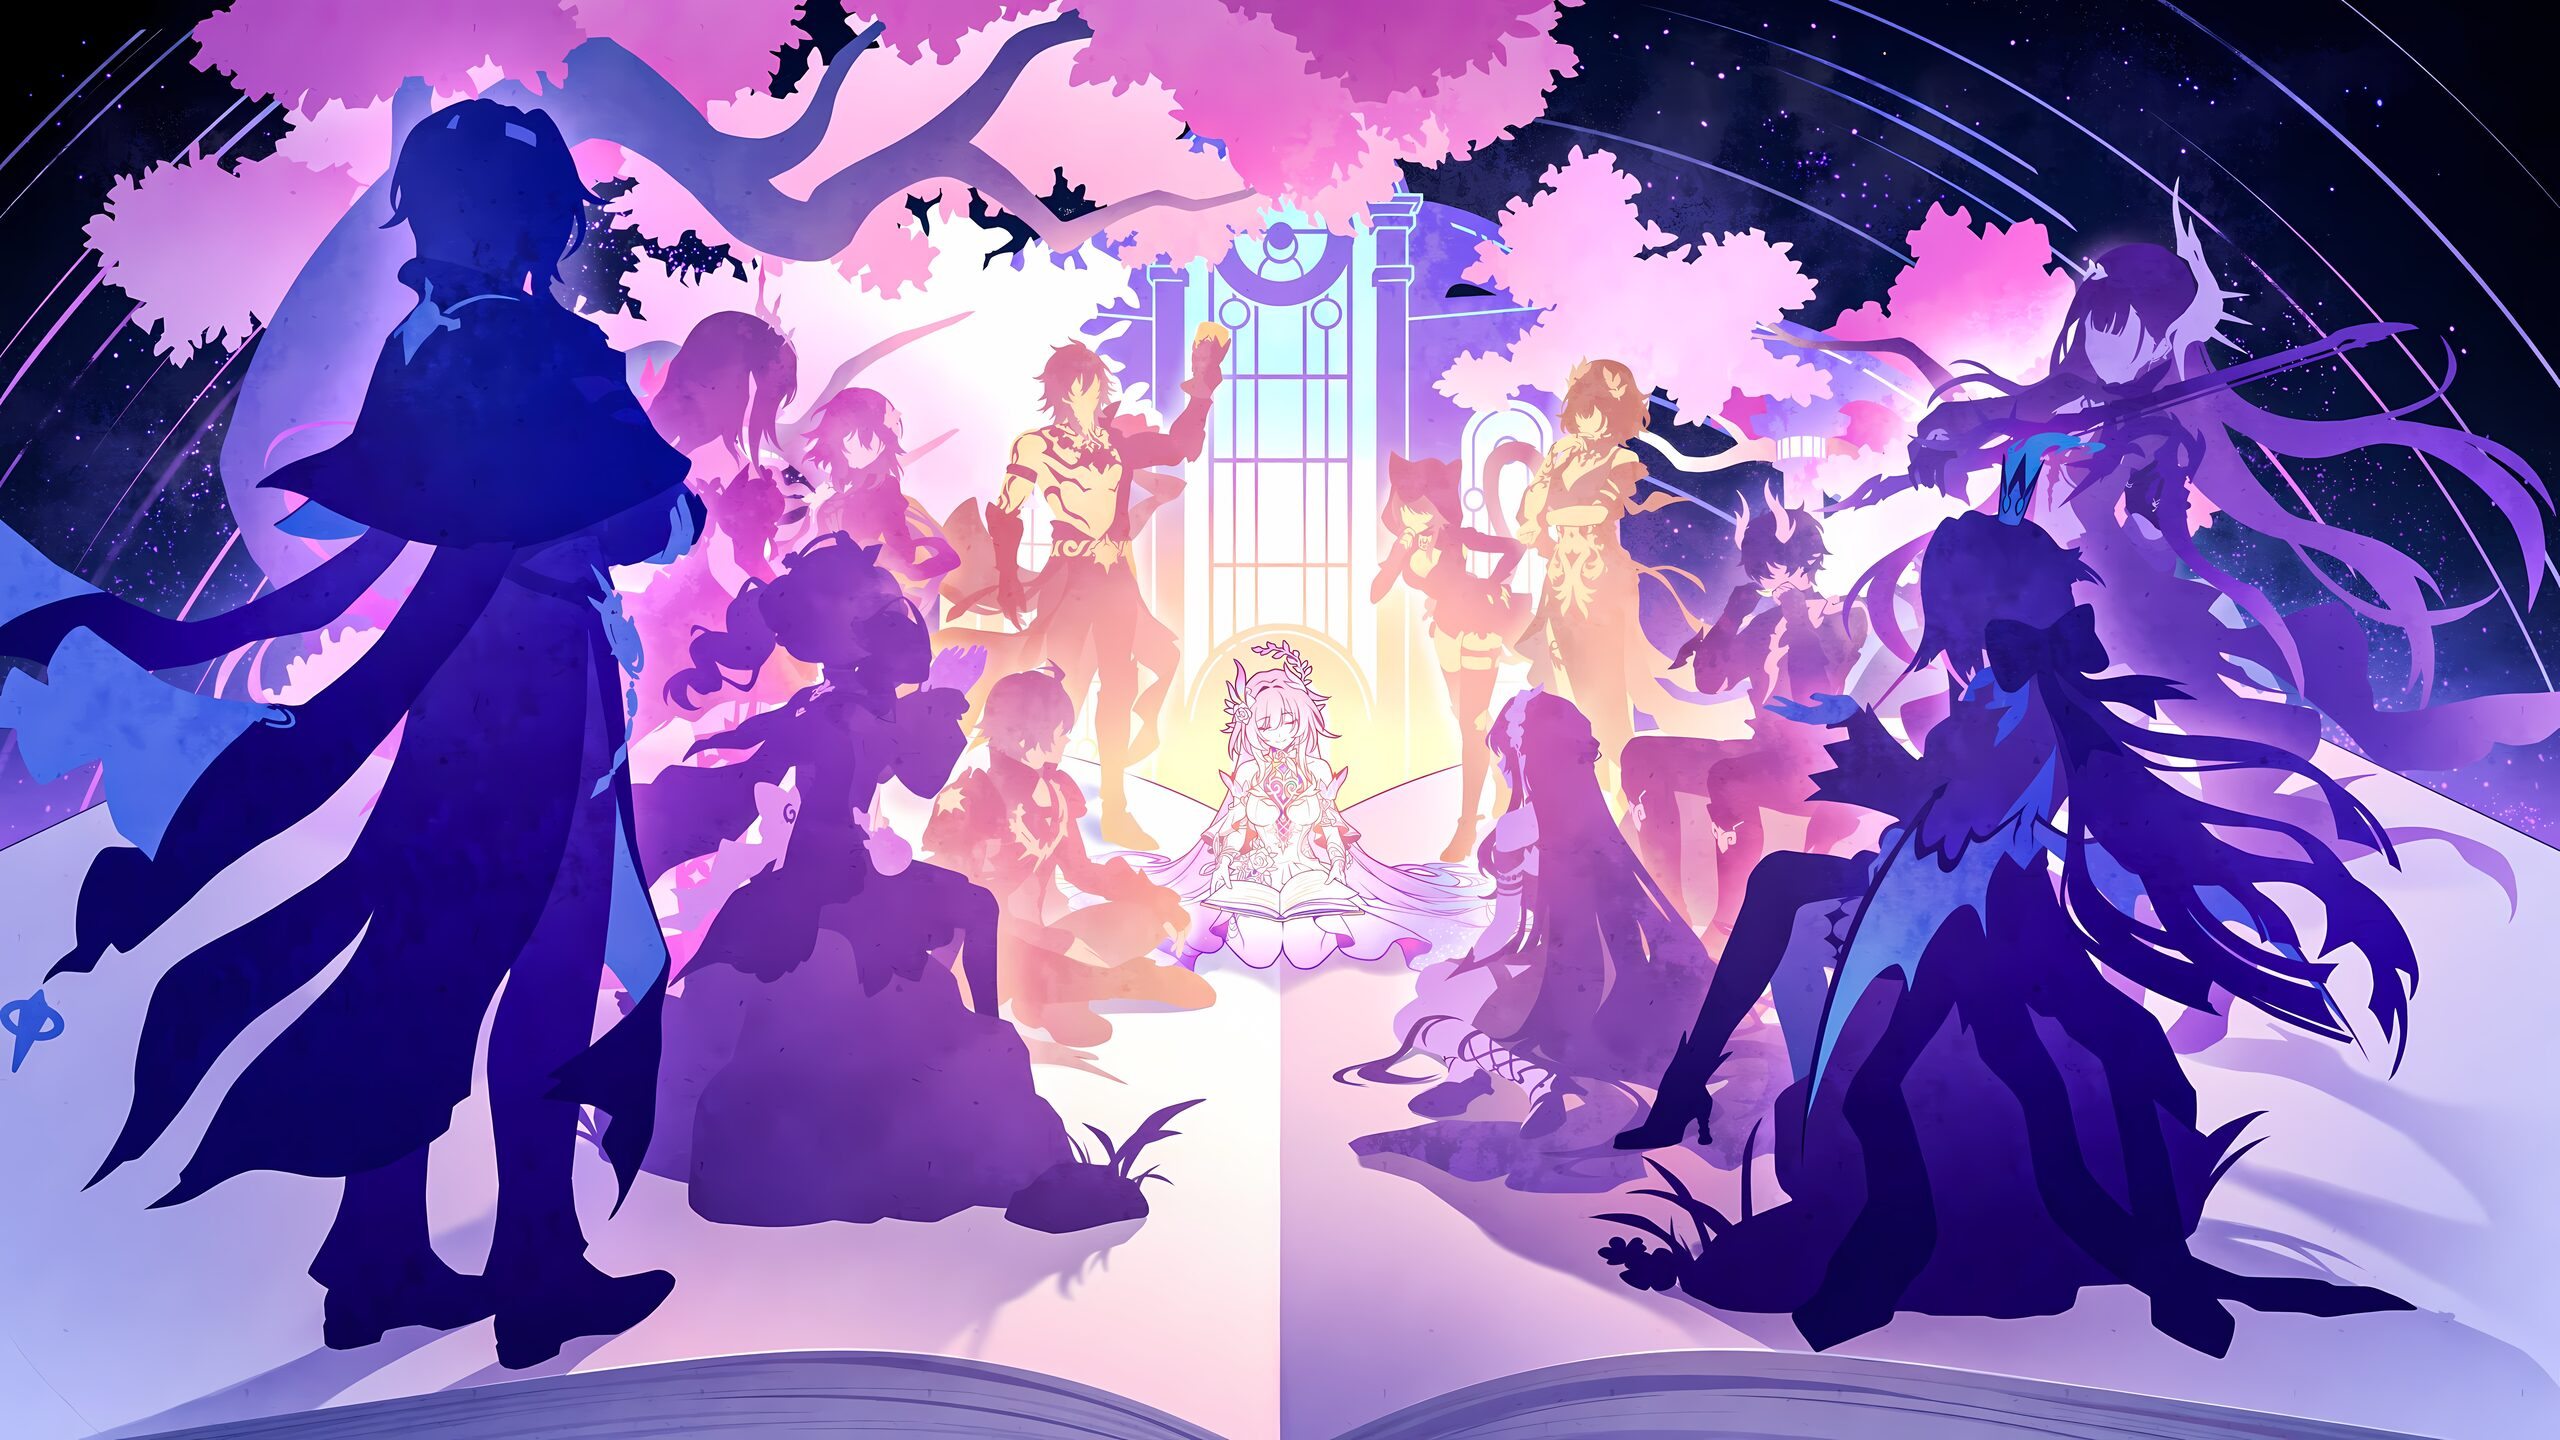
\includegraphics[width=\textwidth,height=0.8\textheight,keepaspectratio]{assets/after.png}
\end{center}
\vspace*{\fill}

\end{document}
